\documentclass[twoside]{book}

% Packages required by doxygen
\usepackage{fixltx2e}
\usepackage{calc}
\usepackage{doxygen}
\usepackage[export]{adjustbox} % also loads graphicx
\usepackage{graphicx}
\usepackage[utf8]{inputenc}
\usepackage{makeidx}
\usepackage{multicol}
\usepackage{multirow}
\PassOptionsToPackage{warn}{textcomp}
\usepackage{textcomp}
\usepackage[nointegrals]{wasysym}
\usepackage[table]{xcolor}

% Font selection
\usepackage[T1]{fontenc}
\usepackage[scaled=.90]{helvet}
\usepackage{courier}
\usepackage{amssymb}
\usepackage{sectsty}
\renewcommand{\familydefault}{\sfdefault}
\allsectionsfont{%
  \fontseries{bc}\selectfont%
  \color{darkgray}%
}
\renewcommand{\DoxyLabelFont}{%
  \fontseries{bc}\selectfont%
  \color{darkgray}%
}
\newcommand{\+}{\discretionary{\mbox{\scriptsize$\hookleftarrow$}}{}{}}

% Page & text layout
\usepackage{geometry}
\geometry{%
  a4paper,%
  top=2.5cm,%
  bottom=2.5cm,%
  left=2.5cm,%
  right=2.5cm%
}
\tolerance=750
\hfuzz=15pt
\hbadness=750
\setlength{\emergencystretch}{15pt}
\setlength{\parindent}{0cm}
\setlength{\parskip}{3ex plus 2ex minus 2ex}
\makeatletter
\renewcommand{\paragraph}{%
  \@startsection{paragraph}{4}{0ex}{-1.0ex}{1.0ex}{%
    \normalfont\normalsize\bfseries\SS@parafont%
  }%
}
\renewcommand{\subparagraph}{%
  \@startsection{subparagraph}{5}{0ex}{-1.0ex}{1.0ex}{%
    \normalfont\normalsize\bfseries\SS@subparafont%
  }%
}
\makeatother

% Headers & footers
\usepackage{fancyhdr}
\pagestyle{fancyplain}
\fancyhead[LE]{\fancyplain{}{\bfseries\thepage}}
\fancyhead[CE]{\fancyplain{}{}}
\fancyhead[RE]{\fancyplain{}{\bfseries\leftmark}}
\fancyhead[LO]{\fancyplain{}{\bfseries\rightmark}}
\fancyhead[CO]{\fancyplain{}{}}
\fancyhead[RO]{\fancyplain{}{\bfseries\thepage}}
\fancyfoot[LE]{\fancyplain{}{}}
\fancyfoot[CE]{\fancyplain{}{}}
\fancyfoot[RE]{\fancyplain{}{\bfseries\scriptsize Generated by Doxygen }}
\fancyfoot[LO]{\fancyplain{}{\bfseries\scriptsize Generated by Doxygen }}
\fancyfoot[CO]{\fancyplain{}{}}
\fancyfoot[RO]{\fancyplain{}{}}
\renewcommand{\footrulewidth}{0.4pt}
\renewcommand{\chaptermark}[1]{%
  \markboth{#1}{}%
}
\renewcommand{\sectionmark}[1]{%
  \markright{\thesection\ #1}%
}

% Indices & bibliography
\usepackage{natbib}
\usepackage[titles]{tocloft}
\setcounter{tocdepth}{3}
\setcounter{secnumdepth}{5}
\makeindex

% Hyperlinks (required, but should be loaded last)
\usepackage{ifpdf}
\ifpdf
  \usepackage[pdftex,pagebackref=true]{hyperref}
\else
  \usepackage[ps2pdf,pagebackref=true]{hyperref}
\fi
\hypersetup{%
  colorlinks=true,%
  linkcolor=blue,%
  citecolor=blue,%
  unicode%
}

% Custom commands
\newcommand{\clearemptydoublepage}{%
  \newpage{\pagestyle{empty}\cleardoublepage}%
}

\usepackage{caption}
\captionsetup{labelsep=space,justification=centering,font={bf},singlelinecheck=off,skip=4pt,position=top}

%===== C O N T E N T S =====

\begin{document}

% Titlepage & ToC
\hypersetup{pageanchor=false,
             bookmarksnumbered=true,
             pdfencoding=unicode
            }
\pagenumbering{alph}
\begin{titlepage}
\vspace*{7cm}
\begin{center}%
{\Large Muon detector \\[1ex]\large 1.\+0 }\\
\vspace*{1cm}
{\large Generated by Doxygen 1.8.13}\\
\end{center}
\end{titlepage}
\clearemptydoublepage
\pagenumbering{roman}
\tableofcontents
\clearemptydoublepage
\pagenumbering{arabic}
\hypersetup{pageanchor=true}

%--- Begin generated contents ---
\chapter{Hierarchical Index}
\section{Class Hierarchy}
This inheritance list is sorted roughly, but not completely, alphabetically\+:\begin{DoxyCompactList}
\item G4\+U\+Imessenger\begin{DoxyCompactList}
\item \contentsline{section}{muon\+Physics\+List\+Messenger}{\pageref{classmuonPhysicsListMessenger}}{}
\end{DoxyCompactList}
\item G4\+User\+Event\+Action\begin{DoxyCompactList}
\item \contentsline{section}{muon\+Event\+Action}{\pageref{classmuonEventAction}}{}
\end{DoxyCompactList}
\item G4\+User\+Run\+Action\begin{DoxyCompactList}
\item \contentsline{section}{muon\+Run\+Action}{\pageref{classmuonRunAction}}{}
\end{DoxyCompactList}
\item G4\+User\+Stepping\+Action\begin{DoxyCompactList}
\item \contentsline{section}{muon\+Stepping\+Action}{\pageref{classmuonSteppingAction}}{}
\end{DoxyCompactList}
\item G4\+V\+Discrete\+Process\begin{DoxyCompactList}
\item \contentsline{section}{muon\+Step\+Max}{\pageref{classmuonStepMax}}{}
\end{DoxyCompactList}
\item G4\+V\+Hit\begin{DoxyCompactList}
\item \contentsline{section}{Energy\+Time\+Hit}{\pageref{classEnergyTimeHit}}{}
\item \contentsline{section}{P\+M\+Thit}{\pageref{classPMThit}}{}
\end{DoxyCompactList}
\item G4\+V\+Modular\+Physics\+List\begin{DoxyCompactList}
\item \contentsline{section}{muon\+Physics\+List}{\pageref{classmuonPhysicsList}}{}
\end{DoxyCompactList}
\item G4\+V\+Physics\+Constructor\begin{DoxyCompactList}
\item \contentsline{section}{muon\+Extra\+Physics}{\pageref{classmuonExtraPhysics}}{}
\item \contentsline{section}{muon\+Optical\+Physics}{\pageref{classmuonOpticalPhysics}}{}
\end{DoxyCompactList}
\item G4\+V\+Sensitive\+Detector\begin{DoxyCompactList}
\item \contentsline{section}{Energy\+Time\+SD}{\pageref{classEnergyTimeSD}}{}
\item \contentsline{section}{pmt\+SD}{\pageref{classpmtSD}}{}
\end{DoxyCompactList}
\item G4\+V\+User\+Action\+Initialization\begin{DoxyCompactList}
\item \contentsline{section}{muon\+Action\+Initialization}{\pageref{classmuonActionInitialization}}{}
\end{DoxyCompactList}
\item G4\+V\+User\+Detector\+Construction\begin{DoxyCompactList}
\item \contentsline{section}{muon\+Detector\+Construction}{\pageref{classmuonDetectorConstruction}}{}
\end{DoxyCompactList}
\item G4\+V\+User\+Primary\+Generator\+Action\begin{DoxyCompactList}
\item \contentsline{section}{muon\+Primary\+Generator\+Action}{\pageref{classmuonPrimaryGeneratorAction}}{}
\end{DoxyCompactList}
\item \contentsline{section}{muon\+Material}{\pageref{classmuonMaterial}}{}
\end{DoxyCompactList}

\chapter{Class Index}
\section{Class List}
Here are the classes, structs, unions and interfaces with brief descriptions\+:\begin{DoxyCompactList}
\item\contentsline{section}{\hyperlink{classEnergyTimeHit}{Energy\+Time\+Hit} \\*设置 Hit 容器 }{\pageref{classEnergyTimeHit}}{}
\item\contentsline{section}{\hyperlink{classEnergyTimeSD}{Energy\+Time\+SD} \\*探测器的敏感探测器类 }{\pageref{classEnergyTimeSD}}{}
\item\contentsline{section}{\hyperlink{classmuonActionInitialization}{muon\+Action\+Initialization} }{\pageref{classmuonActionInitialization}}{}
\item\contentsline{section}{\hyperlink{classmuonDetectorConstruction}{muon\+Detector\+Construction} \\*Detector construction class to define materials and geometry }{\pageref{classmuonDetectorConstruction}}{}
\item\contentsline{section}{\hyperlink{classmuonEventAction}{muon\+Event\+Action} }{\pageref{classmuonEventAction}}{}
\item\contentsline{section}{\hyperlink{classmuonExtraPhysics}{muon\+Extra\+Physics} }{\pageref{classmuonExtraPhysics}}{}
\item\contentsline{section}{\hyperlink{classmuonMaterial}{muon\+Material} }{\pageref{classmuonMaterial}}{}
\item\contentsline{section}{\hyperlink{classmuonOpticalPhysics}{muon\+Optical\+Physics} }{\pageref{classmuonOpticalPhysics}}{}
\item\contentsline{section}{\hyperlink{classmuonPhysicsList}{muon\+Physics\+List} }{\pageref{classmuonPhysicsList}}{}
\item\contentsline{section}{\hyperlink{classmuonPhysicsListMessenger}{muon\+Physics\+List\+Messenger} \\*Provide control of the physics list and cut parameters }{\pageref{classmuonPhysicsListMessenger}}{}
\item\contentsline{section}{\hyperlink{classmuonPrimaryGeneratorAction}{muon\+Primary\+Generator\+Action} }{\pageref{classmuonPrimaryGeneratorAction}}{}
\item\contentsline{section}{\hyperlink{classmuonRunAction}{muon\+Run\+Action} }{\pageref{classmuonRunAction}}{}
\item\contentsline{section}{\hyperlink{classmuonStepMax}{muon\+Step\+Max} }{\pageref{classmuonStepMax}}{}
\item\contentsline{section}{\hyperlink{classmuonSteppingAction}{muon\+Stepping\+Action} }{\pageref{classmuonSteppingAction}}{}
\item\contentsline{section}{\hyperlink{classPMThit}{P\+M\+Thit} \\*设置 Hit 容器 }{\pageref{classPMThit}}{}
\item\contentsline{section}{\hyperlink{classpmtSD}{pmt\+SD} }{\pageref{classpmtSD}}{}
\end{DoxyCompactList}

\chapter{Class Documentation}
\hypertarget{classEnergyTimeHit}{}\section{Energy\+Time\+Hit类 参考}
\label{classEnergyTimeHit}\index{Energy\+Time\+Hit@{Energy\+Time\+Hit}}


设置 muon detector Hit 容器  




{\ttfamily \#include $<$Energy\+Time\+Hit.\+hh$>$}



类 Energy\+Time\+Hit 继承关系图\+:\nopagebreak
\begin{figure}[H]
\begin{center}
\leavevmode
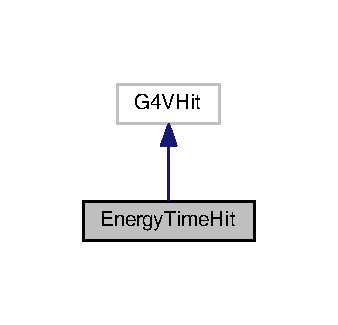
\includegraphics[width=162pt]{classEnergyTimeHit__inherit__graph}
\end{center}
\end{figure}


Energy\+Time\+Hit 的协作图\+:\nopagebreak
\begin{figure}[H]
\begin{center}
\leavevmode
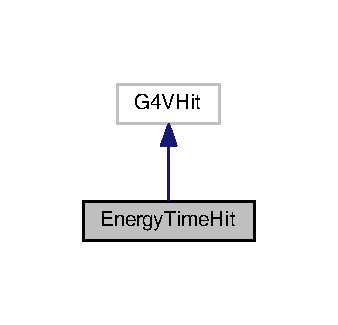
\includegraphics[width=162pt]{classEnergyTimeHit__coll__graph}
\end{center}
\end{figure}
\subsection*{Public 成员函数}
\begin{DoxyCompactItemize}
\item 
void $\ast$ \hyperlink{classEnergyTimeHit_a13352f0fdc7bf25e3655b803b50ae9ca}{operator new} (size\+\_\+t)
\begin{DoxyCompactList}\small\item\em Memory allocation and de-\/allocation \end{DoxyCompactList}\item 
void \hyperlink{classEnergyTimeHit_ab146f5c1aec4e913a416faee3b2ff60b}{operator delete} (void $\ast$)
\item 
void \hyperlink{classEnergyTimeHit_ab7a9602285c51cf42566382df8277147}{Set\+Delta\+Energy} (G4double deltaE)
\begin{DoxyCompactList}\small\item\em 设置能量 \end{DoxyCompactList}\item 
void \hyperlink{classEnergyTimeHit_a139ed317e433a0ddef477117f39daf8a}{Set\+Time} (G4double time)
\begin{DoxyCompactList}\small\item\em 设置时间 \end{DoxyCompactList}\item 
void \hyperlink{classEnergyTimeHit_a987123b85e019adc1f01332bb23c3f2c}{Set\+Position} (G4\+Three\+Vector pos)
\begin{DoxyCompactList}\small\item\em 设置位置 \end{DoxyCompactList}\item 
void \hyperlink{classEnergyTimeHit_aadf608ec3e5d06c9735546b29a0f92b4}{Set\+Name} (G4\+String name)
\begin{DoxyCompactList}\small\item\em 设置探测器名字 \end{DoxyCompactList}\item 
G4double \hyperlink{classEnergyTimeHit_a15aae5ff8efc3a4efc39c00c26308836}{Get\+Delta\+Energy} () const
\begin{DoxyCompactList}\small\item\em 得到 hit 中能量信息 \end{DoxyCompactList}\item 
G4double \hyperlink{classEnergyTimeHit_ab7f49eaf401c5b559876d69330c57c78}{Get\+Time} () const
\begin{DoxyCompactList}\small\item\em 得到 hit 中时间信息 \end{DoxyCompactList}\item 
G4\+Three\+Vector \hyperlink{classEnergyTimeHit_a4611709e7caf2e34f4e368dd8c4e8ad4}{Get\+Position} () const
\begin{DoxyCompactList}\small\item\em 得到 hit 中位置信息 \end{DoxyCompactList}\item 
G4\+String \hyperlink{classEnergyTimeHit_a7e348ee943ce7065910e75b0063108d5}{Get\+Name} () const
\begin{DoxyCompactList}\small\item\em 得到 hit 中探测器信息 \end{DoxyCompactList}\end{DoxyCompactItemize}
\subsection*{Private 属性}
\begin{DoxyCompactItemize}
\item 
G4double \hyperlink{classEnergyTimeHit_a3979f4ac628b68fad49d5014267bbb61}{f\+Delta\+Energy}
\item 
G4double \hyperlink{classEnergyTimeHit_a1c7ce3f598d87ae1855d7edb833d4486}{f\+Time}
\item 
G4\+Three\+Vector \hyperlink{classEnergyTimeHit_adb5230ba263dadd37f343c2c6b04bf55}{f\+Position}
\item 
G4\+String \hyperlink{classEnergyTimeHit_a892c47bfb7d81fe010e7e58413ab52fe}{fname}
\end{DoxyCompactItemize}


\subsection{详细描述}
设置 muon detector Hit 容器 

Hit 容器保存能量,时间,位置,探测器名字 

在文件 Energy\+Time\+Hit.\+hh 第 19 行定义.



\subsection{成员函数说明}
\mbox{\Hypertarget{classEnergyTimeHit_a15aae5ff8efc3a4efc39c00c26308836}\label{classEnergyTimeHit_a15aae5ff8efc3a4efc39c00c26308836}} 
\index{Energy\+Time\+Hit@{Energy\+Time\+Hit}!Get\+Delta\+Energy@{Get\+Delta\+Energy}}
\index{Get\+Delta\+Energy@{Get\+Delta\+Energy}!Energy\+Time\+Hit@{Energy\+Time\+Hit}}
\subsubsection{\texorpdfstring{Get\+Delta\+Energy()}{GetDeltaEnergy()}}
{\footnotesize\ttfamily G4double Energy\+Time\+Hit\+::\+Get\+Delta\+Energy (\begin{DoxyParamCaption}{ }\end{DoxyParamCaption}) const\hspace{0.3cm}{\ttfamily [inline]}}



得到 hit 中能量信息 

在 event\+Action 有用到 

在文件 Energy\+Time\+Hit.\+hh 第 52 行定义.

\mbox{\Hypertarget{classEnergyTimeHit_a7e348ee943ce7065910e75b0063108d5}\label{classEnergyTimeHit_a7e348ee943ce7065910e75b0063108d5}} 
\index{Energy\+Time\+Hit@{Energy\+Time\+Hit}!Get\+Name@{Get\+Name}}
\index{Get\+Name@{Get\+Name}!Energy\+Time\+Hit@{Energy\+Time\+Hit}}
\subsubsection{\texorpdfstring{Get\+Name()}{GetName()}}
{\footnotesize\ttfamily G4\+String Energy\+Time\+Hit\+::\+Get\+Name (\begin{DoxyParamCaption}{ }\end{DoxyParamCaption}) const\hspace{0.3cm}{\ttfamily [inline]}}



得到 hit 中探测器信息 

在 event\+Action 有用到 

在文件 Energy\+Time\+Hit.\+hh 第 67 行定义.

\mbox{\Hypertarget{classEnergyTimeHit_a4611709e7caf2e34f4e368dd8c4e8ad4}\label{classEnergyTimeHit_a4611709e7caf2e34f4e368dd8c4e8ad4}} 
\index{Energy\+Time\+Hit@{Energy\+Time\+Hit}!Get\+Position@{Get\+Position}}
\index{Get\+Position@{Get\+Position}!Energy\+Time\+Hit@{Energy\+Time\+Hit}}
\subsubsection{\texorpdfstring{Get\+Position()}{GetPosition()}}
{\footnotesize\ttfamily G4\+Three\+Vector Energy\+Time\+Hit\+::\+Get\+Position (\begin{DoxyParamCaption}{ }\end{DoxyParamCaption}) const\hspace{0.3cm}{\ttfamily [inline]}}



得到 hit 中位置信息 

在 event\+Action 有用到 

在文件 Energy\+Time\+Hit.\+hh 第 62 行定义.

\mbox{\Hypertarget{classEnergyTimeHit_ab7f49eaf401c5b559876d69330c57c78}\label{classEnergyTimeHit_ab7f49eaf401c5b559876d69330c57c78}} 
\index{Energy\+Time\+Hit@{Energy\+Time\+Hit}!Get\+Time@{Get\+Time}}
\index{Get\+Time@{Get\+Time}!Energy\+Time\+Hit@{Energy\+Time\+Hit}}
\subsubsection{\texorpdfstring{Get\+Time()}{GetTime()}}
{\footnotesize\ttfamily G4double Energy\+Time\+Hit\+::\+Get\+Time (\begin{DoxyParamCaption}{ }\end{DoxyParamCaption}) const\hspace{0.3cm}{\ttfamily [inline]}}



得到 hit 中时间信息 

在 event\+Action 有用到 

在文件 Energy\+Time\+Hit.\+hh 第 57 行定义.

\mbox{\Hypertarget{classEnergyTimeHit_ab146f5c1aec4e913a416faee3b2ff60b}\label{classEnergyTimeHit_ab146f5c1aec4e913a416faee3b2ff60b}} 
\index{Energy\+Time\+Hit@{Energy\+Time\+Hit}!operator delete@{operator delete}}
\index{operator delete@{operator delete}!Energy\+Time\+Hit@{Energy\+Time\+Hit}}
\subsubsection{\texorpdfstring{operator delete()}{operator delete()}}
{\footnotesize\ttfamily void Energy\+Time\+Hit\+::operator delete (\begin{DoxyParamCaption}\item[{void $\ast$}]{a\+Hit }\end{DoxyParamCaption})\hspace{0.3cm}{\ttfamily [inline]}}



在文件 Energy\+Time\+Hit.\+hh 第 89 行定义.

\mbox{\Hypertarget{classEnergyTimeHit_a13352f0fdc7bf25e3655b803b50ae9ca}\label{classEnergyTimeHit_a13352f0fdc7bf25e3655b803b50ae9ca}} 
\index{Energy\+Time\+Hit@{Energy\+Time\+Hit}!operator new@{operator new}}
\index{operator new@{operator new}!Energy\+Time\+Hit@{Energy\+Time\+Hit}}
\subsubsection{\texorpdfstring{operator new()}{operator new()}}
{\footnotesize\ttfamily void $\ast$ Energy\+Time\+Hit\+::operator new (\begin{DoxyParamCaption}\item[{size\+\_\+t}]{ }\end{DoxyParamCaption})\hspace{0.3cm}{\ttfamily [inline]}}



Memory allocation and de-\/allocation 



在文件 Energy\+Time\+Hit.\+hh 第 80 行定义.

\mbox{\Hypertarget{classEnergyTimeHit_ab7a9602285c51cf42566382df8277147}\label{classEnergyTimeHit_ab7a9602285c51cf42566382df8277147}} 
\index{Energy\+Time\+Hit@{Energy\+Time\+Hit}!Set\+Delta\+Energy@{Set\+Delta\+Energy}}
\index{Set\+Delta\+Energy@{Set\+Delta\+Energy}!Energy\+Time\+Hit@{Energy\+Time\+Hit}}
\subsubsection{\texorpdfstring{Set\+Delta\+Energy()}{SetDeltaEnergy()}}
{\footnotesize\ttfamily void Energy\+Time\+Hit\+::\+Set\+Delta\+Energy (\begin{DoxyParamCaption}\item[{G4double}]{deltaE }\end{DoxyParamCaption})\hspace{0.3cm}{\ttfamily [inline]}}



设置能量 


\begin{DoxyParams}{参数}
{\em deltaE} & 在 sensitive类中的\+Process\+Hit()中的从step得到 \\
\hline
\end{DoxyParams}


在文件 Energy\+Time\+Hit.\+hh 第 31 行定义.

\mbox{\Hypertarget{classEnergyTimeHit_aadf608ec3e5d06c9735546b29a0f92b4}\label{classEnergyTimeHit_aadf608ec3e5d06c9735546b29a0f92b4}} 
\index{Energy\+Time\+Hit@{Energy\+Time\+Hit}!Set\+Name@{Set\+Name}}
\index{Set\+Name@{Set\+Name}!Energy\+Time\+Hit@{Energy\+Time\+Hit}}
\subsubsection{\texorpdfstring{Set\+Name()}{SetName()}}
{\footnotesize\ttfamily void Energy\+Time\+Hit\+::\+Set\+Name (\begin{DoxyParamCaption}\item[{G4\+String}]{name }\end{DoxyParamCaption})\hspace{0.3cm}{\ttfamily [inline]}}



设置探测器名字 

因为有两个探测器用一个 logical Volume 所以用这个标记 
\begin{DoxyParams}{参数}
{\em name} & 在 sensitive类中的\+Process\+Hit()中的从step得到 \\
\hline
\end{DoxyParams}


在文件 Energy\+Time\+Hit.\+hh 第 47 行定义.

\mbox{\Hypertarget{classEnergyTimeHit_a987123b85e019adc1f01332bb23c3f2c}\label{classEnergyTimeHit_a987123b85e019adc1f01332bb23c3f2c}} 
\index{Energy\+Time\+Hit@{Energy\+Time\+Hit}!Set\+Position@{Set\+Position}}
\index{Set\+Position@{Set\+Position}!Energy\+Time\+Hit@{Energy\+Time\+Hit}}
\subsubsection{\texorpdfstring{Set\+Position()}{SetPosition()}}
{\footnotesize\ttfamily void Energy\+Time\+Hit\+::\+Set\+Position (\begin{DoxyParamCaption}\item[{G4\+Three\+Vector}]{pos }\end{DoxyParamCaption})\hspace{0.3cm}{\ttfamily [inline]}}



设置位置 


\begin{DoxyParams}{参数}
{\em pos} & 在 sensitive类中的\+Process\+Hit()中的从step得到 \\
\hline
\end{DoxyParams}


在文件 Energy\+Time\+Hit.\+hh 第 41 行定义.

\mbox{\Hypertarget{classEnergyTimeHit_a139ed317e433a0ddef477117f39daf8a}\label{classEnergyTimeHit_a139ed317e433a0ddef477117f39daf8a}} 
\index{Energy\+Time\+Hit@{Energy\+Time\+Hit}!Set\+Time@{Set\+Time}}
\index{Set\+Time@{Set\+Time}!Energy\+Time\+Hit@{Energy\+Time\+Hit}}
\subsubsection{\texorpdfstring{Set\+Time()}{SetTime()}}
{\footnotesize\ttfamily void Energy\+Time\+Hit\+::\+Set\+Time (\begin{DoxyParamCaption}\item[{G4double}]{time }\end{DoxyParamCaption})\hspace{0.3cm}{\ttfamily [inline]}}



设置时间 


\begin{DoxyParams}{参数}
{\em time} & 在 sensitive类中的\+Process\+Hit()中的从step得到 \\
\hline
\end{DoxyParams}


在文件 Energy\+Time\+Hit.\+hh 第 36 行定义.



\subsection{类成员变量说明}
\mbox{\Hypertarget{classEnergyTimeHit_a3979f4ac628b68fad49d5014267bbb61}\label{classEnergyTimeHit_a3979f4ac628b68fad49d5014267bbb61}} 
\index{Energy\+Time\+Hit@{Energy\+Time\+Hit}!f\+Delta\+Energy@{f\+Delta\+Energy}}
\index{f\+Delta\+Energy@{f\+Delta\+Energy}!Energy\+Time\+Hit@{Energy\+Time\+Hit}}
\subsubsection{\texorpdfstring{f\+Delta\+Energy}{fDeltaEnergy}}
{\footnotesize\ttfamily G4double Energy\+Time\+Hit\+::f\+Delta\+Energy\hspace{0.3cm}{\ttfamily [private]}}



在文件 Energy\+Time\+Hit.\+hh 第 69 行定义.

\mbox{\Hypertarget{classEnergyTimeHit_a892c47bfb7d81fe010e7e58413ab52fe}\label{classEnergyTimeHit_a892c47bfb7d81fe010e7e58413ab52fe}} 
\index{Energy\+Time\+Hit@{Energy\+Time\+Hit}!fname@{fname}}
\index{fname@{fname}!Energy\+Time\+Hit@{Energy\+Time\+Hit}}
\subsubsection{\texorpdfstring{fname}{fname}}
{\footnotesize\ttfamily G4\+String Energy\+Time\+Hit\+::fname\hspace{0.3cm}{\ttfamily [private]}}



在文件 Energy\+Time\+Hit.\+hh 第 72 行定义.

\mbox{\Hypertarget{classEnergyTimeHit_adb5230ba263dadd37f343c2c6b04bf55}\label{classEnergyTimeHit_adb5230ba263dadd37f343c2c6b04bf55}} 
\index{Energy\+Time\+Hit@{Energy\+Time\+Hit}!f\+Position@{f\+Position}}
\index{f\+Position@{f\+Position}!Energy\+Time\+Hit@{Energy\+Time\+Hit}}
\subsubsection{\texorpdfstring{f\+Position}{fPosition}}
{\footnotesize\ttfamily G4\+Three\+Vector Energy\+Time\+Hit\+::f\+Position\hspace{0.3cm}{\ttfamily [private]}}



在文件 Energy\+Time\+Hit.\+hh 第 71 行定义.

\mbox{\Hypertarget{classEnergyTimeHit_a1c7ce3f598d87ae1855d7edb833d4486}\label{classEnergyTimeHit_a1c7ce3f598d87ae1855d7edb833d4486}} 
\index{Energy\+Time\+Hit@{Energy\+Time\+Hit}!f\+Time@{f\+Time}}
\index{f\+Time@{f\+Time}!Energy\+Time\+Hit@{Energy\+Time\+Hit}}
\subsubsection{\texorpdfstring{f\+Time}{fTime}}
{\footnotesize\ttfamily G4double Energy\+Time\+Hit\+::f\+Time\hspace{0.3cm}{\ttfamily [private]}}



在文件 Energy\+Time\+Hit.\+hh 第 70 行定义.



该类的文档由以下文件生成\+:\begin{DoxyCompactItemize}
\item 
include/\hyperlink{EnergyTimeHit_8hh}{Energy\+Time\+Hit.\+hh}\end{DoxyCompactItemize}

\hypertarget{classEnergyTimeSD}{}\section{Energy\+Time\+SD Class Reference}
\label{classEnergyTimeSD}\index{Energy\+Time\+SD@{Energy\+Time\+SD}}


探测器的敏感探测器类  




{\ttfamily \#include $<$Energy\+Time\+S\+D.\+hh$>$}



Inheritance diagram for Energy\+Time\+SD\+:\nopagebreak
\begin{figure}[H]
\begin{center}
\leavevmode
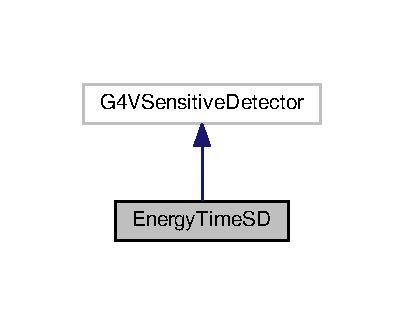
\includegraphics[width=194pt]{classEnergyTimeSD__inherit__graph}
\end{center}
\end{figure}


Collaboration diagram for Energy\+Time\+SD\+:\nopagebreak
\begin{figure}[H]
\begin{center}
\leavevmode
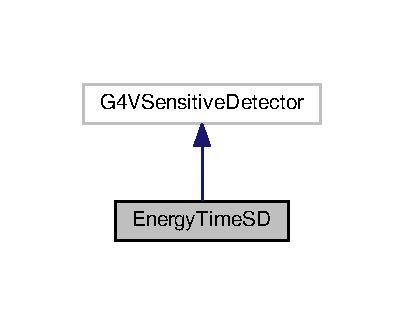
\includegraphics[width=194pt]{classEnergyTimeSD__coll__graph}
\end{center}
\end{figure}
\subsection*{Public Member Functions}
\begin{DoxyCompactItemize}
\item 
\hyperlink{classEnergyTimeSD_a501274766adbbe35de4e8f307ed5b411}{Energy\+Time\+SD} (G4\+String name)
\begin{DoxyCompactList}\small\item\em 构造函数 \end{DoxyCompactList}\item 
void \hyperlink{classEnergyTimeSD_a81809ac7ecdc9eb7bcdc00d489cb9fb3}{Initialize} (G4\+H\+Cof\+This\+Event $\ast$) override
\begin{DoxyCompactList}\small\item\em 初始化敏感探测器 \end{DoxyCompactList}\end{DoxyCompactItemize}
\subsection*{Protected Member Functions}
\begin{DoxyCompactItemize}
\item 
G4bool \hyperlink{classEnergyTimeSD_a24131df6ca564ef0a71e49c4625d5477}{Process\+Hits} (G4\+Step $\ast$a\+Step, G4\+Touchable\+History $\ast$R\+Ohist) override
\begin{DoxyCompactList}\small\item\em 击中敏感探测器处理 \end{DoxyCompactList}\end{DoxyCompactItemize}


\subsection{Detailed Description}
探测器的敏感探测器类 

\subsection{Constructor \& Destructor Documentation}
\mbox{\Hypertarget{classEnergyTimeSD_a501274766adbbe35de4e8f307ed5b411}\label{classEnergyTimeSD_a501274766adbbe35de4e8f307ed5b411}} 
\index{Energy\+Time\+SD@{Energy\+Time\+SD}!Energy\+Time\+SD@{Energy\+Time\+SD}}
\index{Energy\+Time\+SD@{Energy\+Time\+SD}!Energy\+Time\+SD@{Energy\+Time\+SD}}
\subsubsection{\texorpdfstring{Energy\+Time\+S\+D()}{EnergyTimeSD()}}
{\footnotesize\ttfamily Energy\+Time\+S\+D\+::\+Energy\+Time\+SD (\begin{DoxyParamCaption}\item[{G4\+String}]{name }\end{DoxyParamCaption})}



构造函数 

设置敏感探测器保存哪些数据

探测器名字设置

muon 击中敏感探测器,保存时间,能量,位置和击中哪一个探测器信息 敏感探测器挂载在敏感探测器管理类格式为 name/energy\+\_\+time 敏感探测器名字设置

注册管理类时插入 energy\+\_\+time


\begin{DoxyParams}{Parameters}
{\em name} & 敏感探测器的名字 \\
\hline
\end{DoxyParams}


\subsection{Member Function Documentation}
\mbox{\Hypertarget{classEnergyTimeSD_a81809ac7ecdc9eb7bcdc00d489cb9fb3}\label{classEnergyTimeSD_a81809ac7ecdc9eb7bcdc00d489cb9fb3}} 
\index{Energy\+Time\+SD@{Energy\+Time\+SD}!Initialize@{Initialize}}
\index{Initialize@{Initialize}!Energy\+Time\+SD@{Energy\+Time\+SD}}
\subsubsection{\texorpdfstring{Initialize()}{Initialize()}}
{\footnotesize\ttfamily void Energy\+Time\+S\+D\+::\+Initialize (\begin{DoxyParamCaption}\item[{G4\+H\+Cof\+This\+Event $\ast$}]{hcof }\end{DoxyParamCaption})\hspace{0.3cm}{\ttfamily [override]}}



初始化敏感探测器 

将敏感探测器的 id 和 Hit 容器注册到敏感探测器管理类中 \mbox{\Hypertarget{classEnergyTimeSD_a24131df6ca564ef0a71e49c4625d5477}\label{classEnergyTimeSD_a24131df6ca564ef0a71e49c4625d5477}} 
\index{Energy\+Time\+SD@{Energy\+Time\+SD}!Process\+Hits@{Process\+Hits}}
\index{Process\+Hits@{Process\+Hits}!Energy\+Time\+SD@{Energy\+Time\+SD}}
\subsubsection{\texorpdfstring{Process\+Hits()}{ProcessHits()}}
{\footnotesize\ttfamily G4bool Energy\+Time\+S\+D\+::\+Process\+Hits (\begin{DoxyParamCaption}\item[{G4\+Step $\ast$}]{a\+Step,  }\item[{G4\+Touchable\+History $\ast$}]{R\+Ohist }\end{DoxyParamCaption})\hspace{0.3cm}{\ttfamily [override]}, {\ttfamily [protected]}}



击中敏感探测器处理 

将数据保存到 Hit 容器 

The documentation for this class was generated from the following files\+:\begin{DoxyCompactItemize}
\item 
include/Energy\+Time\+S\+D.\+hh\item 
src/Energy\+Time\+S\+D.\+cc\end{DoxyCompactItemize}

\hypertarget{classmuonActionInitialization}{}\section{muon\+Action\+Initialization类 参考}
\label{classmuonActionInitialization}\index{muon\+Action\+Initialization@{muon\+Action\+Initialization}}


action 类的注册  




{\ttfamily \#include $<$muon\+Action\+Initialization.\+hh$>$}



类 muon\+Action\+Initialization 继承关系图\+:\nopagebreak
\begin{figure}[H]
\begin{center}
\leavevmode
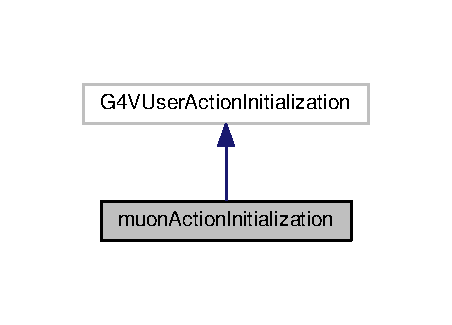
\includegraphics[width=217pt]{classmuonActionInitialization__inherit__graph}
\end{center}
\end{figure}


muon\+Action\+Initialization 的协作图\+:\nopagebreak
\begin{figure}[H]
\begin{center}
\leavevmode
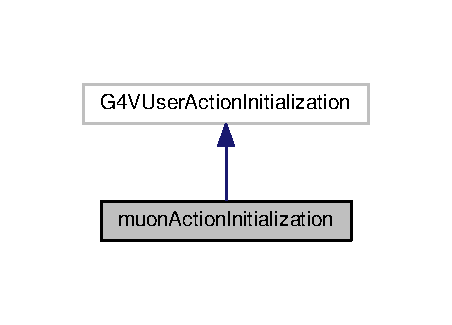
\includegraphics[width=217pt]{classmuonActionInitialization__coll__graph}
\end{center}
\end{figure}
\subsection*{Public 成员函数}
\begin{DoxyCompactItemize}
\item 
\hyperlink{classmuonActionInitialization_ac2975dc863ed514556de9e291a3a655d}{muon\+Action\+Initialization} ()
\begin{DoxyCompactList}\small\item\em 默认 construction 函数 \end{DoxyCompactList}\item 
virtual \hyperlink{classmuonActionInitialization_af86f5507a8d33358f758e1ef65f73597}{$\sim$muon\+Action\+Initialization} ()
\item 
virtual void \hyperlink{classmuonActionInitialization_a6819e8906b517d01966731ccbbac388d}{Build\+For\+Master} () const override
\begin{DoxyCompactList}\small\item\em 多线程 build 暂时没有用 \end{DoxyCompactList}\item 
virtual void \hyperlink{classmuonActionInitialization_afa2c061aba623bc3dcdf417188b17492}{Build} () const override
\begin{DoxyCompactList}\small\item\em 单线程 build \end{DoxyCompactList}\end{DoxyCompactItemize}


\subsection{详细描述}
action 类的注册 

在文件 muon\+Action\+Initialization.\+hh 第 15 行定义.



\subsection{构造及析构函数说明}
\mbox{\Hypertarget{classmuonActionInitialization_ac2975dc863ed514556de9e291a3a655d}\label{classmuonActionInitialization_ac2975dc863ed514556de9e291a3a655d}} 
\index{muon\+Action\+Initialization@{muon\+Action\+Initialization}!muon\+Action\+Initialization@{muon\+Action\+Initialization}}
\index{muon\+Action\+Initialization@{muon\+Action\+Initialization}!muon\+Action\+Initialization@{muon\+Action\+Initialization}}
\subsubsection{\texorpdfstring{muon\+Action\+Initialization()}{muonActionInitialization()}}
{\footnotesize\ttfamily muon\+Action\+Initialization\+::muon\+Action\+Initialization (\begin{DoxyParamCaption}{ }\end{DoxyParamCaption})}



默认 construction 函数 

\mbox{[}long description\mbox{]} 

在文件 muon\+Action\+Initialization.\+cc 第 15 行定义.

\mbox{\Hypertarget{classmuonActionInitialization_af86f5507a8d33358f758e1ef65f73597}\label{classmuonActionInitialization_af86f5507a8d33358f758e1ef65f73597}} 
\index{muon\+Action\+Initialization@{muon\+Action\+Initialization}!````~muon\+Action\+Initialization@{$\sim$muon\+Action\+Initialization}}
\index{````~muon\+Action\+Initialization@{$\sim$muon\+Action\+Initialization}!muon\+Action\+Initialization@{muon\+Action\+Initialization}}
\subsubsection{\texorpdfstring{$\sim$muon\+Action\+Initialization()}{~muonActionInitialization()}}
{\footnotesize\ttfamily muon\+Action\+Initialization\+::$\sim$muon\+Action\+Initialization (\begin{DoxyParamCaption}{ }\end{DoxyParamCaption})\hspace{0.3cm}{\ttfamily [virtual]}}



在文件 muon\+Action\+Initialization.\+cc 第 19 行定义.



\subsection{成员函数说明}
\mbox{\Hypertarget{classmuonActionInitialization_afa2c061aba623bc3dcdf417188b17492}\label{classmuonActionInitialization_afa2c061aba623bc3dcdf417188b17492}} 
\index{muon\+Action\+Initialization@{muon\+Action\+Initialization}!Build@{Build}}
\index{Build@{Build}!muon\+Action\+Initialization@{muon\+Action\+Initialization}}
\subsubsection{\texorpdfstring{Build()}{Build()}}
{\footnotesize\ttfamily void muon\+Action\+Initialization\+::\+Build (\begin{DoxyParamCaption}{ }\end{DoxyParamCaption}) const\hspace{0.3cm}{\ttfamily [override]}, {\ttfamily [virtual]}}



单线程 build 

初始化 \hyperlink{classmuonPrimaryGeneratorAction}{muon\+Primary\+Generator\+Action}, run\+Action,event\+Action,Stepping\+Action 

在文件 muon\+Action\+Initialization.\+cc 第 28 行定义.

\mbox{\Hypertarget{classmuonActionInitialization_a6819e8906b517d01966731ccbbac388d}\label{classmuonActionInitialization_a6819e8906b517d01966731ccbbac388d}} 
\index{muon\+Action\+Initialization@{muon\+Action\+Initialization}!Build\+For\+Master@{Build\+For\+Master}}
\index{Build\+For\+Master@{Build\+For\+Master}!muon\+Action\+Initialization@{muon\+Action\+Initialization}}
\subsubsection{\texorpdfstring{Build\+For\+Master()}{BuildForMaster()}}
{\footnotesize\ttfamily void muon\+Action\+Initialization\+::\+Build\+For\+Master (\begin{DoxyParamCaption}{ }\end{DoxyParamCaption}) const\hspace{0.3cm}{\ttfamily [override]}, {\ttfamily [virtual]}}



多线程 build 暂时没有用 



在文件 muon\+Action\+Initialization.\+cc 第 22 行定义.



该类的文档由以下文件生成\+:\begin{DoxyCompactItemize}
\item 
include/\hyperlink{muonActionInitialization_8hh}{muon\+Action\+Initialization.\+hh}\item 
src/\hyperlink{muonActionInitialization_8cc}{muon\+Action\+Initialization.\+cc}\end{DoxyCompactItemize}

\hypertarget{classmuonDetectorConstruction}{}\section{muon\+Detector\+Construction Class Reference}
\label{classmuonDetectorConstruction}\index{muon\+Detector\+Construction@{muon\+Detector\+Construction}}


Detector construction class to define materials and geometry.  




{\ttfamily \#include $<$muon\+Detector\+Construction.\+hh$>$}



Inheritance diagram for muon\+Detector\+Construction\+:\nopagebreak
\begin{figure}[H]
\begin{center}
\leavevmode
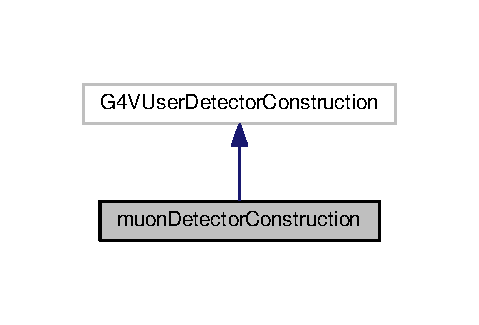
\includegraphics[width=230pt]{classmuonDetectorConstruction__inherit__graph}
\end{center}
\end{figure}


Collaboration diagram for muon\+Detector\+Construction\+:\nopagebreak
\begin{figure}[H]
\begin{center}
\leavevmode
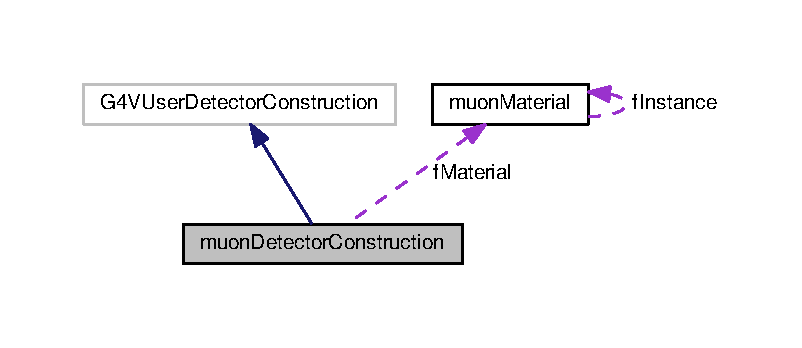
\includegraphics[width=230pt]{classmuonDetectorConstruction__coll__graph}
\end{center}
\end{figure}
\subsection*{Public Member Functions}
\begin{DoxyCompactItemize}
\item 
\mbox{\Hypertarget{classmuonDetectorConstruction_ad2b397202446a2fb7d563a8122cd5ecc}\label{classmuonDetectorConstruction_ad2b397202446a2fb7d563a8122cd5ecc}} 
\hyperlink{classmuonDetectorConstruction_ad2b397202446a2fb7d563a8122cd5ecc}{muon\+Detector\+Construction} ()
\begin{DoxyCompactList}\small\item\em 搭建探测器 \end{DoxyCompactList}\item 
\mbox{\Hypertarget{classmuonDetectorConstruction_ae06d0e4ad5f07bc1465a7faeccfdd19d}\label{classmuonDetectorConstruction_ae06d0e4ad5f07bc1465a7faeccfdd19d}} 
virtual G4\+V\+Physical\+Volume $\ast$ {\bfseries Construct} () override
\item 
\mbox{\Hypertarget{classmuonDetectorConstruction_a1f76a4cb61622b57c22e2041afb96181}\label{classmuonDetectorConstruction_a1f76a4cb61622b57c22e2041afb96181}} 
void {\bfseries Constructmuondetector} (G4\+Logical\+Volume $\ast$)
\item 
\mbox{\Hypertarget{classmuonDetectorConstruction_aa5c57ff26fa5e8339698103cf5422dd8}\label{classmuonDetectorConstruction_aa5c57ff26fa5e8339698103cf5422dd8}} 
void {\bfseries Construct\+P\+MT} (G4\+Logical\+Volume $\ast$)
\item 
\mbox{\Hypertarget{classmuonDetectorConstruction_a01081b09828848dd76666d4e59cbab52}\label{classmuonDetectorConstruction_a01081b09828848dd76666d4e59cbab52}} 
void {\bfseries Construct\+Reflection} (G4\+Logical\+Volume $\ast$, G4\+Trd $\ast$)
\item 
\mbox{\Hypertarget{classmuonDetectorConstruction_ab730c9af042466f6464c77a62a3c75df}\label{classmuonDetectorConstruction_ab730c9af042466f6464c77a62a3c75df}} 
void {\bfseries Construct\+S\+Dand\+Field} () override
\end{DoxyCompactItemize}


\subsection{Detailed Description}
Detector construction class to define materials and geometry. 

The documentation for this class was generated from the following files\+:\begin{DoxyCompactItemize}
\item 
include/muon\+Detector\+Construction.\+hh\item 
src/muon\+Detector\+Construction.\+cc\end{DoxyCompactItemize}

\hypertarget{classmuonEventAction}{}\section{muon\+Event\+Action类 参考}
\label{classmuonEventAction}\index{muon\+Event\+Action@{muon\+Event\+Action}}


保存信息输出到 Ntuple  




{\ttfamily \#include $<$muon\+Event\+Action.\+hh$>$}



类 muon\+Event\+Action 继承关系图\+:\nopagebreak
\begin{figure}[H]
\begin{center}
\leavevmode
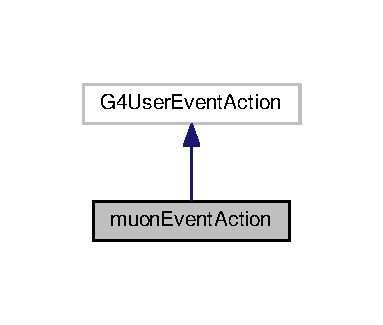
\includegraphics[width=184pt]{classmuonEventAction__inherit__graph}
\end{center}
\end{figure}


muon\+Event\+Action 的协作图\+:\nopagebreak
\begin{figure}[H]
\begin{center}
\leavevmode
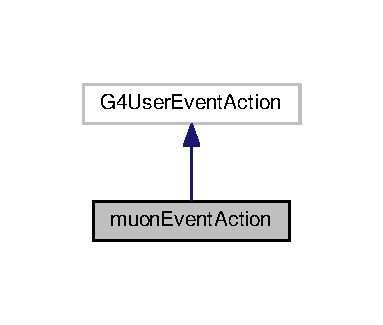
\includegraphics[width=184pt]{classmuonEventAction__coll__graph}
\end{center}
\end{figure}
\subsection*{Public 成员函数}
\begin{DoxyCompactItemize}
\item 
\hyperlink{classmuonEventAction_a5584cb4df883c49fb98b082aacf0a269}{muon\+Event\+Action} ()
\begin{DoxyCompactList}\small\item\em 默认 construction 函数 \end{DoxyCompactList}\item 
virtual \hyperlink{classmuonEventAction_ae268609426bf99b1459f72e21215fdc4}{$\sim$muon\+Event\+Action} ()
\item 
virtual void \hyperlink{classmuonEventAction_a674e82851a04669f19294aae5e4a69e6}{End\+Of\+Event\+Action} (const G4\+Event $\ast$an\+Event) override
\begin{DoxyCompactList}\small\item\em 保存信息到 Ntuple 中 \end{DoxyCompactList}\end{DoxyCompactItemize}
\subsection*{Private 属性}
\begin{DoxyCompactItemize}
\item 
G4int \hyperlink{classmuonEventAction_a16fc4814b4d56184e4e458b5b9c5b8b7}{muondetector\+En\+Id} \{ -\/1 \}
\item 
G4int \hyperlink{classmuonEventAction_a569d9e868f1be3db60bcc7ef512a3b7f}{P\+M\+T\+\_\+\+Id} \{-\/1\}
\end{DoxyCompactItemize}


\subsection{详细描述}
保存信息输出到 Ntuple 

在文件 muon\+Event\+Action.\+hh 第 18 行定义.



\subsection{构造及析构函数说明}
\mbox{\Hypertarget{classmuonEventAction_a5584cb4df883c49fb98b082aacf0a269}\label{classmuonEventAction_a5584cb4df883c49fb98b082aacf0a269}} 
\index{muon\+Event\+Action@{muon\+Event\+Action}!muon\+Event\+Action@{muon\+Event\+Action}}
\index{muon\+Event\+Action@{muon\+Event\+Action}!muon\+Event\+Action@{muon\+Event\+Action}}
\subsubsection{\texorpdfstring{muon\+Event\+Action()}{muonEventAction()}}
{\footnotesize\ttfamily muon\+Event\+Action\+::muon\+Event\+Action (\begin{DoxyParamCaption}{ }\end{DoxyParamCaption})}



默认 construction 函数 



在文件 muon\+Event\+Action.\+cc 第 20 行定义.

\mbox{\Hypertarget{classmuonEventAction_ae268609426bf99b1459f72e21215fdc4}\label{classmuonEventAction_ae268609426bf99b1459f72e21215fdc4}} 
\index{muon\+Event\+Action@{muon\+Event\+Action}!````~muon\+Event\+Action@{$\sim$muon\+Event\+Action}}
\index{````~muon\+Event\+Action@{$\sim$muon\+Event\+Action}!muon\+Event\+Action@{muon\+Event\+Action}}
\subsubsection{\texorpdfstring{$\sim$muon\+Event\+Action()}{~muonEventAction()}}
{\footnotesize\ttfamily muon\+Event\+Action\+::$\sim$muon\+Event\+Action (\begin{DoxyParamCaption}{ }\end{DoxyParamCaption})\hspace{0.3cm}{\ttfamily [virtual]}}



在文件 muon\+Event\+Action.\+cc 第 23 行定义.



\subsection{成员函数说明}
\mbox{\Hypertarget{classmuonEventAction_a674e82851a04669f19294aae5e4a69e6}\label{classmuonEventAction_a674e82851a04669f19294aae5e4a69e6}} 
\index{muon\+Event\+Action@{muon\+Event\+Action}!End\+Of\+Event\+Action@{End\+Of\+Event\+Action}}
\index{End\+Of\+Event\+Action@{End\+Of\+Event\+Action}!muon\+Event\+Action@{muon\+Event\+Action}}
\subsubsection{\texorpdfstring{End\+Of\+Event\+Action()}{EndOfEventAction()}}
{\footnotesize\ttfamily void muon\+Event\+Action\+::\+End\+Of\+Event\+Action (\begin{DoxyParamCaption}\item[{const G4\+Event $\ast$}]{an\+Event }\end{DoxyParamCaption})\hspace{0.3cm}{\ttfamily [override]}, {\ttfamily [virtual]}}



保存信息到 Ntuple 中 

获得敏感探测器的 id, 输出数据

保存 pmt hitcollection 和 muon detector hitcollection 
\begin{DoxyParams}{参数}
{\em an\+Event} & \mbox{[}description\mbox{]} \\
\hline
\end{DoxyParams}
第一列 能量 第二列 时间 第三列 如果是 探测器 ‘\+P\+M\+T1\textquotesingle{} 则为 1, 探测器 ’\+P\+M\+T2‘ 则为 2 第四列 event id

第一列 能量 第二列 深度信息 第三列 如果是 探测器 ‘muondector1\textquotesingle{} 则为 1, 探测器 ’muondector2‘ 则为 2 第四列 event id

在文件 muon\+Event\+Action.\+cc 第 29 行定义.



\subsection{类成员变量说明}
\mbox{\Hypertarget{classmuonEventAction_a16fc4814b4d56184e4e458b5b9c5b8b7}\label{classmuonEventAction_a16fc4814b4d56184e4e458b5b9c5b8b7}} 
\index{muon\+Event\+Action@{muon\+Event\+Action}!muondetector\+En\+Id@{muondetector\+En\+Id}}
\index{muondetector\+En\+Id@{muondetector\+En\+Id}!muon\+Event\+Action@{muon\+Event\+Action}}
\subsubsection{\texorpdfstring{muondetector\+En\+Id}{muondetectorEnId}}
{\footnotesize\ttfamily G4int muon\+Event\+Action\+::muondetector\+En\+Id \{ -\/1 \}\hspace{0.3cm}{\ttfamily [private]}}



在文件 muon\+Event\+Action.\+hh 第 34 行定义.

\mbox{\Hypertarget{classmuonEventAction_a569d9e868f1be3db60bcc7ef512a3b7f}\label{classmuonEventAction_a569d9e868f1be3db60bcc7ef512a3b7f}} 
\index{muon\+Event\+Action@{muon\+Event\+Action}!P\+M\+T\+\_\+\+Id@{P\+M\+T\+\_\+\+Id}}
\index{P\+M\+T\+\_\+\+Id@{P\+M\+T\+\_\+\+Id}!muon\+Event\+Action@{muon\+Event\+Action}}
\subsubsection{\texorpdfstring{P\+M\+T\+\_\+\+Id}{PMT\_Id}}
{\footnotesize\ttfamily G4int muon\+Event\+Action\+::\+P\+M\+T\+\_\+\+Id \{-\/1\}\hspace{0.3cm}{\ttfamily [private]}}



在文件 muon\+Event\+Action.\+hh 第 35 行定义.



该类的文档由以下文件生成\+:\begin{DoxyCompactItemize}
\item 
include/\hyperlink{muonEventAction_8hh}{muon\+Event\+Action.\+hh}\item 
src/\hyperlink{muonEventAction_8cc}{muon\+Event\+Action.\+cc}\end{DoxyCompactItemize}

\hypertarget{classmuonExtraPhysics}{}\section{muon\+Extra\+Physics Class Reference}
\label{classmuonExtraPhysics}\index{muon\+Extra\+Physics@{muon\+Extra\+Physics}}


Inheritance diagram for muon\+Extra\+Physics\+:\nopagebreak
\begin{figure}[H]
\begin{center}
\leavevmode
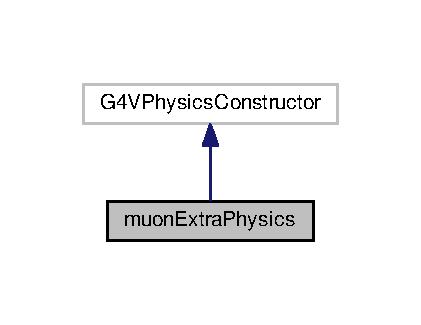
\includegraphics[width=202pt]{classmuonExtraPhysics__inherit__graph}
\end{center}
\end{figure}


Collaboration diagram for muon\+Extra\+Physics\+:\nopagebreak
\begin{figure}[H]
\begin{center}
\leavevmode
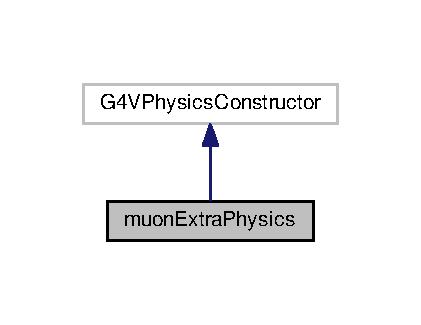
\includegraphics[width=202pt]{classmuonExtraPhysics__coll__graph}
\end{center}
\end{figure}
\subsection*{Public Member Functions}
\begin{DoxyCompactItemize}
\item 
\mbox{\Hypertarget{classmuonExtraPhysics_a499780469ca3774cc90f6a73bc750f1e}\label{classmuonExtraPhysics_a499780469ca3774cc90f6a73bc750f1e}} 
virtual void {\bfseries Construct\+Particle} ()
\item 
\mbox{\Hypertarget{classmuonExtraPhysics_acd8e6a94a2520746e6ae7cf342b83db5}\label{classmuonExtraPhysics_acd8e6a94a2520746e6ae7cf342b83db5}} 
virtual void {\bfseries Construct\+Process} ()
\end{DoxyCompactItemize}


The documentation for this class was generated from the following files\+:\begin{DoxyCompactItemize}
\item 
include/muon\+Extra\+Physics.\+hh\item 
src/muon\+Extra\+Physics.\+cc\end{DoxyCompactItemize}

\hypertarget{classmuonMaterial}{}\section{muon\+Material类 参考}
\label{classmuonMaterial}\index{muon\+Material@{muon\+Material}}


构建材料  




{\ttfamily \#include $<$muon\+Material.\+hh$>$}



muon\+Material 的协作图\+:\nopagebreak
\begin{figure}[H]
\begin{center}
\leavevmode
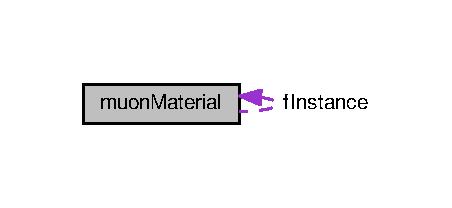
\includegraphics[width=217pt]{classmuonMaterial__coll__graph}
\end{center}
\end{figure}
\subsection*{Public 成员函数}
\begin{DoxyCompactItemize}
\item 
\hyperlink{classmuonMaterial_ae18416f718e33ca4a8bf12b11fe7d4cf}{muon\+Material} ()
\begin{DoxyCompactList}\small\item\em 默认 construction 函数并初始化 f\+Nist\+Man \end{DoxyCompactList}\item 
\hyperlink{classmuonMaterial_a4f043be3ac0578d37c1c2cd801b9a1d8}{$\sim$muon\+Material} ()
\item 
G4\+Material $\ast$ \hyperlink{classmuonMaterial_a86cd49b45dd1042b6ec7aa697197c0b5}{Get\+Material} (const G4\+String)
\begin{DoxyCompactList}\small\item\em 根据名字找到 nist 下的材料 \end{DoxyCompactList}\item 
G4\+Material $\ast$ \hyperlink{classmuonMaterial_a8621980c58fd47d46f47728850341aa5}{Getfdetector} ()
\begin{DoxyCompactList}\small\item\em 得到 detector 的材料 \end{DoxyCompactList}\item 
G4\+Material $\ast$ \hyperlink{classmuonMaterial_a198ba1027e11cf15bc0118533fff4356}{Getf\+P\+MT} ()
\begin{DoxyCompactList}\small\item\em 得到 P\+MT 的材料 \end{DoxyCompactList}\item 
G4\+Material $\ast$ \hyperlink{classmuonMaterial_a8b1a5528153587650e3990045cae47a1}{Getfreflect} ()
\begin{DoxyCompactList}\small\item\em 得到 reflect 的材料 \end{DoxyCompactList}\item 
G4\+Material $\ast$ \hyperlink{classmuonMaterial_a561de210ea339679872c522163990899}{Getf\+Air} ()
\begin{DoxyCompactList}\small\item\em 得到 world 的材料-\/空气 \end{DoxyCompactList}\end{DoxyCompactItemize}
\subsection*{静态 Public 成员函数}
\begin{DoxyCompactItemize}
\item 
static \hyperlink{classmuonMaterial}{muon\+Material} $\ast$ \hyperlink{classmuonMaterial_ac5be4443f4de88103fea67e651cc554b}{Get\+Instance} ()
\end{DoxyCompactItemize}
\subsection*{Private 成员函数}
\begin{DoxyCompactItemize}
\item 
void \hyperlink{classmuonMaterial_a8a540dd90dc8252913e5dcb63d7f07b0}{Create\+Materials} ()
\begin{DoxyCompactList}\small\item\em 构建材料 \end{DoxyCompactList}\end{DoxyCompactItemize}
\subsection*{Private 属性}
\begin{DoxyCompactItemize}
\item 
G4\+Nist\+Manager $\ast$ \hyperlink{classmuonMaterial_a369d8b63868ac68fc917aa93cc321d17}{f\+Nist\+Man}
\item 
G4\+Material $\ast$ \hyperlink{classmuonMaterial_ae5df2e697057d4e3c7e22f1152942eb4}{fdetector}
\item 
G4\+Material $\ast$ \hyperlink{classmuonMaterial_a91b124a58e862152b3a04317d3ca8cbc}{f\+P\+MT}
\item 
G4\+Material $\ast$ \hyperlink{classmuonMaterial_a62687d2a8459169ed8c79aaedaf9013d}{freflect}
\item 
G4\+Material $\ast$ \hyperlink{classmuonMaterial_aad484f194b194516ad00b9c263345639}{f\+Air}
\end{DoxyCompactItemize}
\subsection*{静态 Private 属性}
\begin{DoxyCompactItemize}
\item 
static \hyperlink{classmuonMaterial}{muon\+Material} $\ast$ \hyperlink{classmuonMaterial_a930e3601f3476643cc24db541f6ea253}{f\+Instance} =0
\end{DoxyCompactItemize}


\subsection{详细描述}
构建材料 

在文件 muon\+Material.\+hh 第 17 行定义.



\subsection{构造及析构函数说明}
\mbox{\Hypertarget{classmuonMaterial_ae18416f718e33ca4a8bf12b11fe7d4cf}\label{classmuonMaterial_ae18416f718e33ca4a8bf12b11fe7d4cf}} 
\index{muon\+Material@{muon\+Material}!muon\+Material@{muon\+Material}}
\index{muon\+Material@{muon\+Material}!muon\+Material@{muon\+Material}}
\subsubsection{\texorpdfstring{muon\+Material()}{muonMaterial()}}
{\footnotesize\ttfamily muon\+Material\+::muon\+Material (\begin{DoxyParamCaption}{ }\end{DoxyParamCaption})}



默认 construction 函数并初始化 f\+Nist\+Man 



在文件 muon\+Material.\+cc 第 13 行定义.

\mbox{\Hypertarget{classmuonMaterial_a4f043be3ac0578d37c1c2cd801b9a1d8}\label{classmuonMaterial_a4f043be3ac0578d37c1c2cd801b9a1d8}} 
\index{muon\+Material@{muon\+Material}!````~muon\+Material@{$\sim$muon\+Material}}
\index{````~muon\+Material@{$\sim$muon\+Material}!muon\+Material@{muon\+Material}}
\subsubsection{\texorpdfstring{$\sim$muon\+Material()}{~muonMaterial()}}
{\footnotesize\ttfamily muon\+Material\+::$\sim$muon\+Material (\begin{DoxyParamCaption}{ }\end{DoxyParamCaption})}



在文件 muon\+Material.\+cc 第 21 行定义.



\subsection{成员函数说明}
\mbox{\Hypertarget{classmuonMaterial_a8a540dd90dc8252913e5dcb63d7f07b0}\label{classmuonMaterial_a8a540dd90dc8252913e5dcb63d7f07b0}} 
\index{muon\+Material@{muon\+Material}!Create\+Materials@{Create\+Materials}}
\index{Create\+Materials@{Create\+Materials}!muon\+Material@{muon\+Material}}
\subsubsection{\texorpdfstring{Create\+Materials()}{CreateMaterials()}}
{\footnotesize\ttfamily void muon\+Material\+::\+Create\+Materials (\begin{DoxyParamCaption}{ }\end{DoxyParamCaption})\hspace{0.3cm}{\ttfamily [private]}}



构建材料 

初始化 fdetector f\+P\+MT freflect f\+Air 

在文件 muon\+Material.\+cc 第 53 行定义.

\mbox{\Hypertarget{classmuonMaterial_a561de210ea339679872c522163990899}\label{classmuonMaterial_a561de210ea339679872c522163990899}} 
\index{muon\+Material@{muon\+Material}!Getf\+Air@{Getf\+Air}}
\index{Getf\+Air@{Getf\+Air}!muon\+Material@{muon\+Material}}
\subsubsection{\texorpdfstring{Getf\+Air()}{GetfAir()}}
{\footnotesize\ttfamily G4\+Material$\ast$ muon\+Material\+::\+Getf\+Air (\begin{DoxyParamCaption}{ }\end{DoxyParamCaption})\hspace{0.3cm}{\ttfamily [inline]}}



得到 world 的材料-\/空气 

\begin{DoxyReturn}{返回}
world 的材料 
\end{DoxyReturn}


在文件 muon\+Material.\+hh 第 48 行定义.

\mbox{\Hypertarget{classmuonMaterial_a8621980c58fd47d46f47728850341aa5}\label{classmuonMaterial_a8621980c58fd47d46f47728850341aa5}} 
\index{muon\+Material@{muon\+Material}!Getfdetector@{Getfdetector}}
\index{Getfdetector@{Getfdetector}!muon\+Material@{muon\+Material}}
\subsubsection{\texorpdfstring{Getfdetector()}{Getfdetector()}}
{\footnotesize\ttfamily G4\+Material$\ast$ muon\+Material\+::\+Getfdetector (\begin{DoxyParamCaption}{ }\end{DoxyParamCaption})\hspace{0.3cm}{\ttfamily [inline]}}



得到 detector 的材料 

\begin{DoxyReturn}{返回}
detector 的材料 
\end{DoxyReturn}


在文件 muon\+Material.\+hh 第 33 行定义.

\mbox{\Hypertarget{classmuonMaterial_a198ba1027e11cf15bc0118533fff4356}\label{classmuonMaterial_a198ba1027e11cf15bc0118533fff4356}} 
\index{muon\+Material@{muon\+Material}!Getf\+P\+MT@{Getf\+P\+MT}}
\index{Getf\+P\+MT@{Getf\+P\+MT}!muon\+Material@{muon\+Material}}
\subsubsection{\texorpdfstring{Getf\+P\+M\+T()}{GetfPMT()}}
{\footnotesize\ttfamily G4\+Material$\ast$ muon\+Material\+::\+Getf\+P\+MT (\begin{DoxyParamCaption}{ }\end{DoxyParamCaption})\hspace{0.3cm}{\ttfamily [inline]}}



得到 P\+MT 的材料 

\begin{DoxyReturn}{返回}
P\+MT 的材料 
\end{DoxyReturn}


在文件 muon\+Material.\+hh 第 38 行定义.

\mbox{\Hypertarget{classmuonMaterial_a8b1a5528153587650e3990045cae47a1}\label{classmuonMaterial_a8b1a5528153587650e3990045cae47a1}} 
\index{muon\+Material@{muon\+Material}!Getfreflect@{Getfreflect}}
\index{Getfreflect@{Getfreflect}!muon\+Material@{muon\+Material}}
\subsubsection{\texorpdfstring{Getfreflect()}{Getfreflect()}}
{\footnotesize\ttfamily G4\+Material$\ast$ muon\+Material\+::\+Getfreflect (\begin{DoxyParamCaption}{ }\end{DoxyParamCaption})\hspace{0.3cm}{\ttfamily [inline]}}



得到 reflect 的材料 

\begin{DoxyReturn}{返回}
reflect 的材料 
\end{DoxyReturn}


在文件 muon\+Material.\+hh 第 43 行定义.

\mbox{\Hypertarget{classmuonMaterial_ac5be4443f4de88103fea67e651cc554b}\label{classmuonMaterial_ac5be4443f4de88103fea67e651cc554b}} 
\index{muon\+Material@{muon\+Material}!Get\+Instance@{Get\+Instance}}
\index{Get\+Instance@{Get\+Instance}!muon\+Material@{muon\+Material}}
\subsubsection{\texorpdfstring{Get\+Instance()}{GetInstance()}}
{\footnotesize\ttfamily \hyperlink{classmuonMaterial}{muon\+Material} $\ast$ muon\+Material\+::\+Get\+Instance (\begin{DoxyParamCaption}{ }\end{DoxyParamCaption})\hspace{0.3cm}{\ttfamily [static]}}



在文件 muon\+Material.\+cc 第 27 行定义.

\mbox{\Hypertarget{classmuonMaterial_a86cd49b45dd1042b6ec7aa697197c0b5}\label{classmuonMaterial_a86cd49b45dd1042b6ec7aa697197c0b5}} 
\index{muon\+Material@{muon\+Material}!Get\+Material@{Get\+Material}}
\index{Get\+Material@{Get\+Material}!muon\+Material@{muon\+Material}}
\subsubsection{\texorpdfstring{Get\+Material()}{GetMaterial()}}
{\footnotesize\ttfamily G4\+Material $\ast$ muon\+Material\+::\+Get\+Material (\begin{DoxyParamCaption}\item[{const G4\+String}]{material }\end{DoxyParamCaption})}



根据名字找到 nist 下的材料 



在文件 muon\+Material.\+cc 第 36 行定义.



\subsection{类成员变量说明}
\mbox{\Hypertarget{classmuonMaterial_aad484f194b194516ad00b9c263345639}\label{classmuonMaterial_aad484f194b194516ad00b9c263345639}} 
\index{muon\+Material@{muon\+Material}!f\+Air@{f\+Air}}
\index{f\+Air@{f\+Air}!muon\+Material@{muon\+Material}}
\subsubsection{\texorpdfstring{f\+Air}{fAir}}
{\footnotesize\ttfamily G4\+Material$\ast$ muon\+Material\+::f\+Air\hspace{0.3cm}{\ttfamily [private]}}



在文件 muon\+Material.\+hh 第 66 行定义.

\mbox{\Hypertarget{classmuonMaterial_ae5df2e697057d4e3c7e22f1152942eb4}\label{classmuonMaterial_ae5df2e697057d4e3c7e22f1152942eb4}} 
\index{muon\+Material@{muon\+Material}!fdetector@{fdetector}}
\index{fdetector@{fdetector}!muon\+Material@{muon\+Material}}
\subsubsection{\texorpdfstring{fdetector}{fdetector}}
{\footnotesize\ttfamily G4\+Material$\ast$ muon\+Material\+::fdetector\hspace{0.3cm}{\ttfamily [private]}}



在文件 muon\+Material.\+hh 第 63 行定义.

\mbox{\Hypertarget{classmuonMaterial_a930e3601f3476643cc24db541f6ea253}\label{classmuonMaterial_a930e3601f3476643cc24db541f6ea253}} 
\index{muon\+Material@{muon\+Material}!f\+Instance@{f\+Instance}}
\index{f\+Instance@{f\+Instance}!muon\+Material@{muon\+Material}}
\subsubsection{\texorpdfstring{f\+Instance}{fInstance}}
{\footnotesize\ttfamily \hyperlink{classmuonMaterial}{muon\+Material} $\ast$ muon\+Material\+::f\+Instance =0\hspace{0.3cm}{\ttfamily [static]}, {\ttfamily [private]}}



在文件 muon\+Material.\+hh 第 59 行定义.

\mbox{\Hypertarget{classmuonMaterial_a369d8b63868ac68fc917aa93cc321d17}\label{classmuonMaterial_a369d8b63868ac68fc917aa93cc321d17}} 
\index{muon\+Material@{muon\+Material}!f\+Nist\+Man@{f\+Nist\+Man}}
\index{f\+Nist\+Man@{f\+Nist\+Man}!muon\+Material@{muon\+Material}}
\subsubsection{\texorpdfstring{f\+Nist\+Man}{fNistMan}}
{\footnotesize\ttfamily G4\+Nist\+Manager$\ast$ muon\+Material\+::f\+Nist\+Man\hspace{0.3cm}{\ttfamily [private]}}



在文件 muon\+Material.\+hh 第 61 行定义.

\mbox{\Hypertarget{classmuonMaterial_a91b124a58e862152b3a04317d3ca8cbc}\label{classmuonMaterial_a91b124a58e862152b3a04317d3ca8cbc}} 
\index{muon\+Material@{muon\+Material}!f\+P\+MT@{f\+P\+MT}}
\index{f\+P\+MT@{f\+P\+MT}!muon\+Material@{muon\+Material}}
\subsubsection{\texorpdfstring{f\+P\+MT}{fPMT}}
{\footnotesize\ttfamily G4\+Material$\ast$ muon\+Material\+::f\+P\+MT\hspace{0.3cm}{\ttfamily [private]}}



在文件 muon\+Material.\+hh 第 64 行定义.

\mbox{\Hypertarget{classmuonMaterial_a62687d2a8459169ed8c79aaedaf9013d}\label{classmuonMaterial_a62687d2a8459169ed8c79aaedaf9013d}} 
\index{muon\+Material@{muon\+Material}!freflect@{freflect}}
\index{freflect@{freflect}!muon\+Material@{muon\+Material}}
\subsubsection{\texorpdfstring{freflect}{freflect}}
{\footnotesize\ttfamily G4\+Material$\ast$ muon\+Material\+::freflect\hspace{0.3cm}{\ttfamily [private]}}



在文件 muon\+Material.\+hh 第 65 行定义.



该类的文档由以下文件生成\+:\begin{DoxyCompactItemize}
\item 
include/\hyperlink{muonMaterial_8hh}{muon\+Material.\+hh}\item 
src/\hyperlink{muonMaterial_8cc}{muon\+Material.\+cc}\end{DoxyCompactItemize}

\hypertarget{classmuonOpticalPhysics}{}\section{muon\+Optical\+Physics Class Reference}
\label{classmuonOpticalPhysics}\index{muon\+Optical\+Physics@{muon\+Optical\+Physics}}


Inheritance diagram for muon\+Optical\+Physics\+:\nopagebreak
\begin{figure}[H]
\begin{center}
\leavevmode
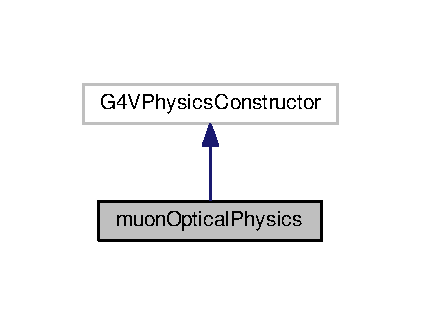
\includegraphics[width=202pt]{classmuonOpticalPhysics__inherit__graph}
\end{center}
\end{figure}


Collaboration diagram for muon\+Optical\+Physics\+:\nopagebreak
\begin{figure}[H]
\begin{center}
\leavevmode
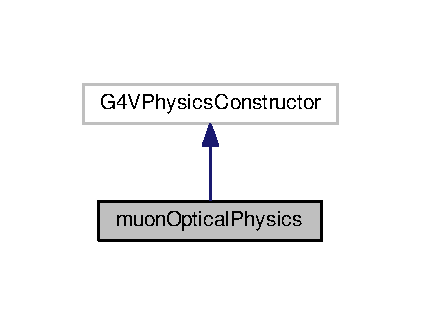
\includegraphics[width=202pt]{classmuonOpticalPhysics__coll__graph}
\end{center}
\end{figure}
\subsection*{Public Member Functions}
\begin{DoxyCompactItemize}
\item 
\mbox{\Hypertarget{classmuonOpticalPhysics_a52eeca699e5ceef8bbf6b7e6aa2911d8}\label{classmuonOpticalPhysics_a52eeca699e5ceef8bbf6b7e6aa2911d8}} 
{\bfseries muon\+Optical\+Physics} (G4bool toggle=true)
\item 
\mbox{\Hypertarget{classmuonOpticalPhysics_a0d4026c22223e1cbe9c4db0e4d45699d}\label{classmuonOpticalPhysics_a0d4026c22223e1cbe9c4db0e4d45699d}} 
virtual void {\bfseries Construct\+Particle} ()
\item 
\mbox{\Hypertarget{classmuonOpticalPhysics_aee337a42afb4af85865cde2e460e120f}\label{classmuonOpticalPhysics_aee337a42afb4af85865cde2e460e120f}} 
virtual void {\bfseries Construct\+Process} ()
\item 
\mbox{\Hypertarget{classmuonOpticalPhysics_a257a178b6e1a98c10d9001fe43d0b1c8}\label{classmuonOpticalPhysics_a257a178b6e1a98c10d9001fe43d0b1c8}} 
G4\+Op\+W\+LS $\ast$ {\bfseries Get\+W\+L\+S\+Process} ()
\item 
\mbox{\Hypertarget{classmuonOpticalPhysics_a6588a993cc57cade05bb1371c60bf914}\label{classmuonOpticalPhysics_a6588a993cc57cade05bb1371c60bf914}} 
G4\+Cerenkov $\ast$ {\bfseries Get\+Cerenkov\+Process} ()
\item 
\mbox{\Hypertarget{classmuonOpticalPhysics_acda9b8ac8d073939523c861833c343ce}\label{classmuonOpticalPhysics_acda9b8ac8d073939523c861833c343ce}} 
G4\+Scintillation $\ast$ {\bfseries Get\+Scintillation\+Process} ()
\item 
\mbox{\Hypertarget{classmuonOpticalPhysics_a0e66d292a9509fdc6703fcdea0e38c7d}\label{classmuonOpticalPhysics_a0e66d292a9509fdc6703fcdea0e38c7d}} 
G4\+Op\+Absorption $\ast$ {\bfseries Get\+Absorption\+Process} ()
\item 
\mbox{\Hypertarget{classmuonOpticalPhysics_a443ff15987bae9b5d07155252f7fad9b}\label{classmuonOpticalPhysics_a443ff15987bae9b5d07155252f7fad9b}} 
G4\+Op\+Rayleigh $\ast$ {\bfseries Get\+Rayleigh\+Scattering\+Process} ()
\item 
\mbox{\Hypertarget{classmuonOpticalPhysics_a57eae82cad6cd757dd6e283598a4bf54}\label{classmuonOpticalPhysics_a57eae82cad6cd757dd6e283598a4bf54}} 
G4\+Op\+Mie\+HG $\ast$ {\bfseries Get\+Mie\+H\+G\+Scattering\+Process} ()
\item 
\mbox{\Hypertarget{classmuonOpticalPhysics_ad1abfb3c7d0cea07d456c5651390b168}\label{classmuonOpticalPhysics_ad1abfb3c7d0cea07d456c5651390b168}} 
G4\+Op\+Boundary\+Process $\ast$ {\bfseries Get\+Boundary\+Process} ()
\item 
\mbox{\Hypertarget{classmuonOpticalPhysics_a99125ac76dc52e14be98e0a1326d3f71}\label{classmuonOpticalPhysics_a99125ac76dc52e14be98e0a1326d3f71}} 
void {\bfseries Set\+Nb\+Of\+Photons\+Cerenkov} (G4int)
\end{DoxyCompactItemize}


The documentation for this class was generated from the following files\+:\begin{DoxyCompactItemize}
\item 
include/muon\+Optical\+Physics.\+hh\item 
src/muon\+Optical\+Physics.\+cc\end{DoxyCompactItemize}

\hypertarget{classmuonPhysicsList}{}\section{muon\+Physics\+List Class Reference}
\label{classmuonPhysicsList}\index{muon\+Physics\+List@{muon\+Physics\+List}}


Inheritance diagram for muon\+Physics\+List\+:\nopagebreak
\begin{figure}[H]
\begin{center}
\leavevmode
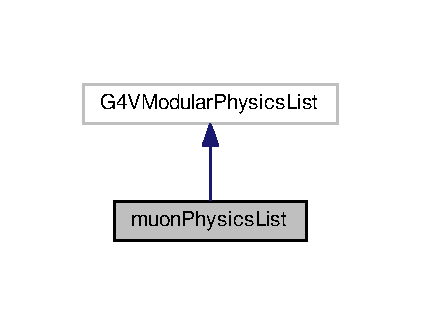
\includegraphics[width=202pt]{classmuonPhysicsList__inherit__graph}
\end{center}
\end{figure}


Collaboration diagram for muon\+Physics\+List\+:\nopagebreak
\begin{figure}[H]
\begin{center}
\leavevmode
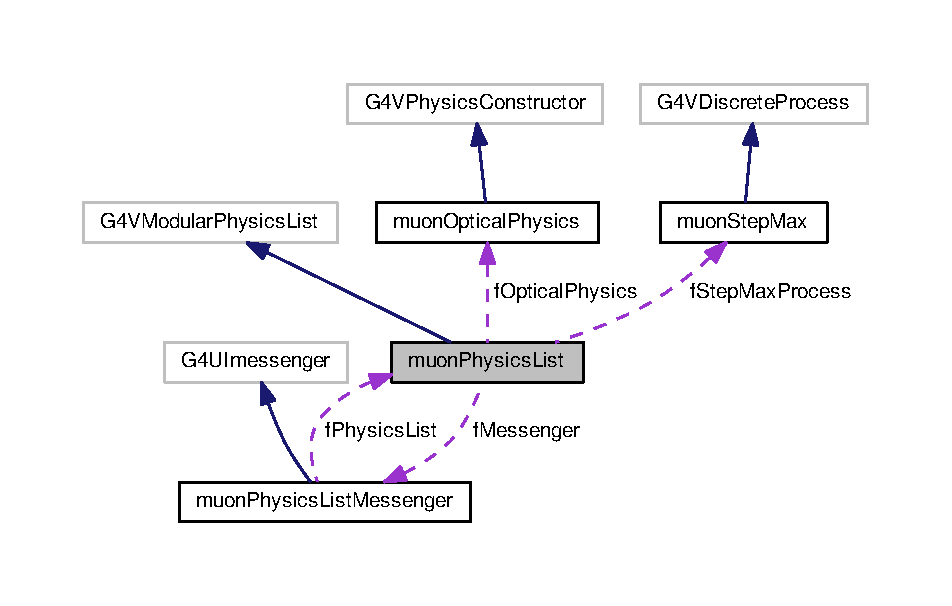
\includegraphics[width=202pt]{classmuonPhysicsList__coll__graph}
\end{center}
\end{figure}
\subsection*{Public Member Functions}
\begin{DoxyCompactItemize}
\item 
\mbox{\Hypertarget{classmuonPhysicsList_aec1adc0f09839b739713b95b60a3433c}\label{classmuonPhysicsList_aec1adc0f09839b739713b95b60a3433c}} 
{\bfseries muon\+Physics\+List} (G4\+String)
\item 
\mbox{\Hypertarget{classmuonPhysicsList_ae567a51ca4aff57c7148bb3886bff6d0}\label{classmuonPhysicsList_ae567a51ca4aff57c7148bb3886bff6d0}} 
void {\bfseries Set\+Cuts} ()
\item 
\mbox{\Hypertarget{classmuonPhysicsList_a462e709c365cb2c502eba1c71fb24d06}\label{classmuonPhysicsList_a462e709c365cb2c502eba1c71fb24d06}} 
void {\bfseries Set\+Cut\+For\+Gamma} (G4double)
\item 
\mbox{\Hypertarget{classmuonPhysicsList_a0d5e15f23de27e9ed9876eb9fb481b7f}\label{classmuonPhysicsList_a0d5e15f23de27e9ed9876eb9fb481b7f}} 
void {\bfseries Set\+Cut\+For\+Electron} (G4double)
\item 
\mbox{\Hypertarget{classmuonPhysicsList_a610582e1c0d233f2c5c0914189547d08}\label{classmuonPhysicsList_a610582e1c0d233f2c5c0914189547d08}} 
void {\bfseries Set\+Cut\+For\+Positron} (G4double)
\item 
\mbox{\Hypertarget{classmuonPhysicsList_a43f30e66e8518d33040777262bbc829f}\label{classmuonPhysicsList_a43f30e66e8518d33040777262bbc829f}} 
void {\bfseries Set\+Step\+Max} (G4double)
\item 
\mbox{\Hypertarget{classmuonPhysicsList_a673fde0059508d78547a84db91971ce9}\label{classmuonPhysicsList_a673fde0059508d78547a84db91971ce9}} 
\hyperlink{classmuonStepMax}{muon\+Step\+Max} $\ast$ {\bfseries Get\+Step\+Max\+Process} ()
\item 
\mbox{\Hypertarget{classmuonPhysicsList_a9d96538f586114bd672f975658527527}\label{classmuonPhysicsList_a9d96538f586114bd672f975658527527}} 
void {\bfseries Add\+Step\+Max} ()
\item 
\mbox{\Hypertarget{classmuonPhysicsList_aaba742da0c9dc44a6498bfc804e284eb}\label{classmuonPhysicsList_aaba742da0c9dc44a6498bfc804e284eb}} 
void \hyperlink{classmuonPhysicsList_aaba742da0c9dc44a6498bfc804e284eb}{Remove\+From\+Physics\+List} (const G4\+String \&)
\begin{DoxyCompactList}\small\item\em Remove specific physics from physics list. \end{DoxyCompactList}\item 
\mbox{\Hypertarget{classmuonPhysicsList_a4a34c6141040c0d5bd34396df7d10ff3}\label{classmuonPhysicsList_a4a34c6141040c0d5bd34396df7d10ff3}} 
void \hyperlink{classmuonPhysicsList_a4a34c6141040c0d5bd34396df7d10ff3}{Clear\+Physics} ()
\begin{DoxyCompactList}\small\item\em Make sure that the physics list is empty. \end{DoxyCompactList}\item 
\mbox{\Hypertarget{classmuonPhysicsList_aefb2f75ee5958cfcf78b50c479523703}\label{classmuonPhysicsList_aefb2f75ee5958cfcf78b50c479523703}} 
virtual void {\bfseries Construct\+Particle} ()
\item 
\mbox{\Hypertarget{classmuonPhysicsList_aac0f8e3bd5e0509f96613e150554d06e}\label{classmuonPhysicsList_aac0f8e3bd5e0509f96613e150554d06e}} 
virtual void {\bfseries Construct\+Process} ()
\item 
\mbox{\Hypertarget{classmuonPhysicsList_afe6f5f4bcf37f721cd821753ace0b06d}\label{classmuonPhysicsList_afe6f5f4bcf37f721cd821753ace0b06d}} 
void {\bfseries Set\+Absorption} (G4bool)
\item 
\mbox{\Hypertarget{classmuonPhysicsList_abf3b923807c3112086ea15a698d5666b}\label{classmuonPhysicsList_abf3b923807c3112086ea15a698d5666b}} 
void {\bfseries Set\+Nb\+Of\+Photons\+Cerenkov} (G4int)
\item 
\mbox{\Hypertarget{classmuonPhysicsList_a459c2902a6bf45261961a67954324c9b}\label{classmuonPhysicsList_a459c2902a6bf45261961a67954324c9b}} 
void {\bfseries Set\+Verbose} (G4int)
\end{DoxyCompactItemize}


The documentation for this class was generated from the following files\+:\begin{DoxyCompactItemize}
\item 
include/muon\+Physics\+List.\+hh\item 
src/muon\+Physics\+List.\+cc\end{DoxyCompactItemize}

\hypertarget{classmuonPhysicsListMessenger}{}\section{muon\+Physics\+List\+Messenger Class Reference}
\label{classmuonPhysicsListMessenger}\index{muon\+Physics\+List\+Messenger@{muon\+Physics\+List\+Messenger}}


Provide control of the physics list and cut parameters.  




{\ttfamily \#include $<$muon\+Physics\+List\+Messenger.\+hh$>$}



Inheritance diagram for muon\+Physics\+List\+Messenger\+:\nopagebreak
\begin{figure}[H]
\begin{center}
\leavevmode
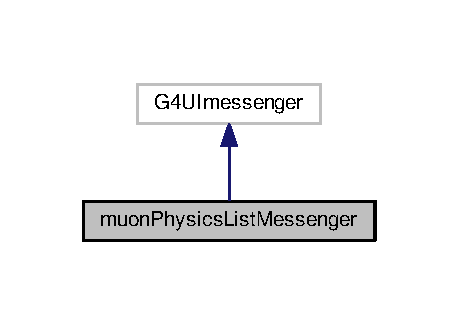
\includegraphics[width=220pt]{classmuonPhysicsListMessenger__inherit__graph}
\end{center}
\end{figure}


Collaboration diagram for muon\+Physics\+List\+Messenger\+:\nopagebreak
\begin{figure}[H]
\begin{center}
\leavevmode
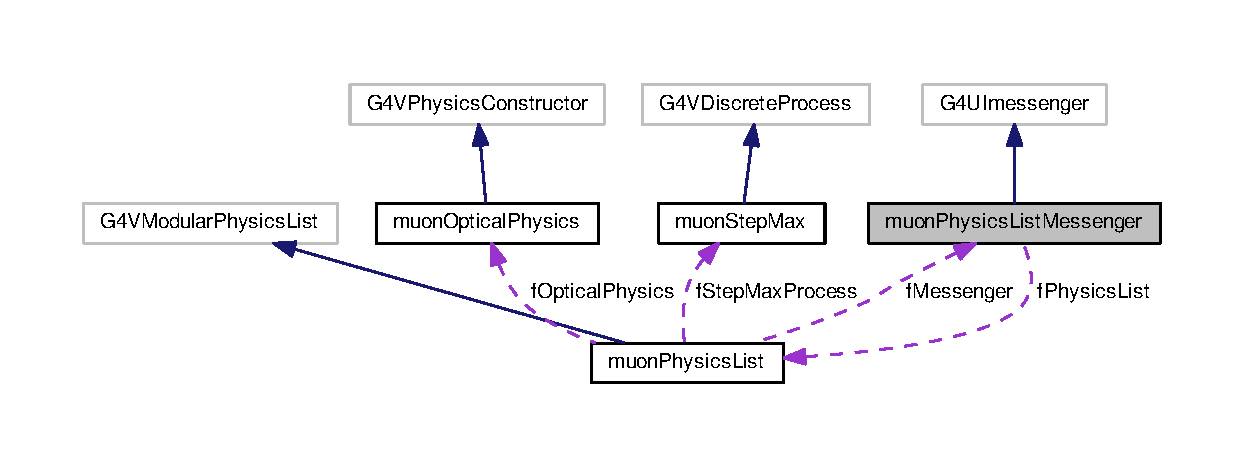
\includegraphics[width=220pt]{classmuonPhysicsListMessenger__coll__graph}
\end{center}
\end{figure}
\subsection*{Public Member Functions}
\begin{DoxyCompactItemize}
\item 
\mbox{\Hypertarget{classmuonPhysicsListMessenger_a11858a3a5031e4e9b36a2f92906d992f}\label{classmuonPhysicsListMessenger_a11858a3a5031e4e9b36a2f92906d992f}} 
{\bfseries muon\+Physics\+List\+Messenger} (\hyperlink{classmuonPhysicsList}{muon\+Physics\+List} $\ast$)
\item 
\mbox{\Hypertarget{classmuonPhysicsListMessenger_a89644cda40ed2e4fa88f2344a7bbedc4}\label{classmuonPhysicsListMessenger_a89644cda40ed2e4fa88f2344a7bbedc4}} 
virtual void {\bfseries Set\+New\+Value} (G4\+U\+Icommand $\ast$, G4\+String)
\end{DoxyCompactItemize}


\subsection{Detailed Description}
Provide control of the physics list and cut parameters. 

The documentation for this class was generated from the following files\+:\begin{DoxyCompactItemize}
\item 
include/muon\+Physics\+List\+Messenger.\+hh\item 
src/muon\+Physics\+List\+Messenger.\+cc\end{DoxyCompactItemize}

\hypertarget{classmuonPrimaryGeneratorAction}{}\section{muon\+Primary\+Generator\+Action Class Reference}
\label{classmuonPrimaryGeneratorAction}\index{muon\+Primary\+Generator\+Action@{muon\+Primary\+Generator\+Action}}


Inheritance diagram for muon\+Primary\+Generator\+Action\+:\nopagebreak
\begin{figure}[H]
\begin{center}
\leavevmode
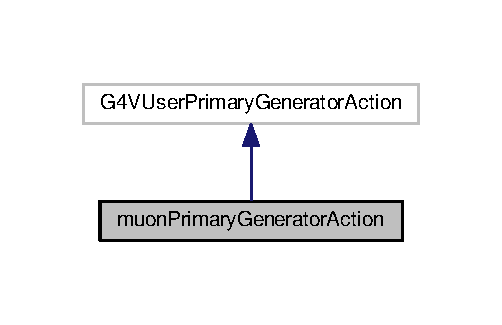
\includegraphics[width=241pt]{classmuonPrimaryGeneratorAction__inherit__graph}
\end{center}
\end{figure}


Collaboration diagram for muon\+Primary\+Generator\+Action\+:\nopagebreak
\begin{figure}[H]
\begin{center}
\leavevmode
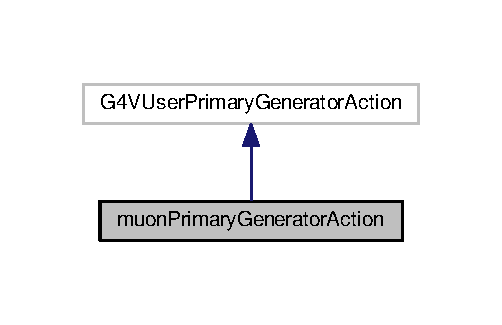
\includegraphics[width=241pt]{classmuonPrimaryGeneratorAction__coll__graph}
\end{center}
\end{figure}
\subsection*{Public Member Functions}
\begin{DoxyCompactItemize}
\item 
\mbox{\Hypertarget{classmuonPrimaryGeneratorAction_a885d97924b9fcb69292c33eafb314c60}\label{classmuonPrimaryGeneratorAction_a885d97924b9fcb69292c33eafb314c60}} 
virtual void {\bfseries Generate\+Primaries} (G4\+Event $\ast$an\+Event) override
\item 
\mbox{\Hypertarget{classmuonPrimaryGeneratorAction_a2a8edec5c700a748aefbd2ec2a95157a}\label{classmuonPrimaryGeneratorAction_a2a8edec5c700a748aefbd2ec2a95157a}} 
const G4\+Particle\+Gun $\ast$ {\bfseries Get\+Particle\+Gun} () const
\end{DoxyCompactItemize}


The documentation for this class was generated from the following files\+:\begin{DoxyCompactItemize}
\item 
include/muon\+Primary\+Generator\+Action.\+hh\item 
src/muon\+Primary\+Generator\+Action.\+cc\end{DoxyCompactItemize}

\hypertarget{classmuonRunAction}{}\section{muon\+Run\+Action Class Reference}
\label{classmuonRunAction}\index{muon\+Run\+Action@{muon\+Run\+Action}}


Inheritance diagram for muon\+Run\+Action\+:\nopagebreak
\begin{figure}[H]
\begin{center}
\leavevmode
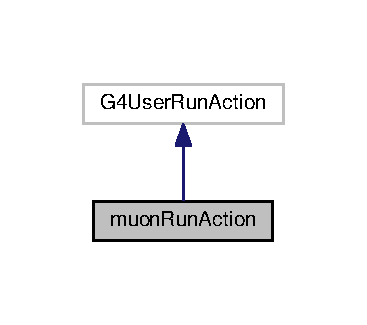
\includegraphics[width=176pt]{classmuonRunAction__inherit__graph}
\end{center}
\end{figure}


Collaboration diagram for muon\+Run\+Action\+:\nopagebreak
\begin{figure}[H]
\begin{center}
\leavevmode
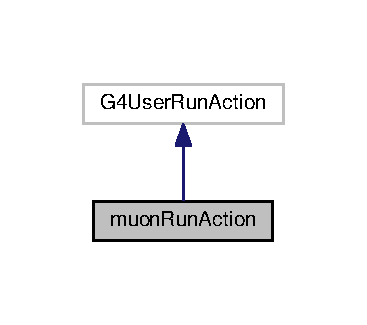
\includegraphics[width=176pt]{classmuonRunAction__coll__graph}
\end{center}
\end{figure}
\subsection*{Public Member Functions}
\begin{DoxyCompactItemize}
\item 
\mbox{\Hypertarget{classmuonRunAction_af8ea0396dde7e9a638382c7134173929}\label{classmuonRunAction_af8ea0396dde7e9a638382c7134173929}} 
\hyperlink{classmuonRunAction_af8ea0396dde7e9a638382c7134173929}{muon\+Run\+Action} ()
\begin{DoxyCompactList}\small\item\em 打开 csv 文件,文件名,声明哪些数据被保存 \end{DoxyCompactList}\item 
\mbox{\Hypertarget{classmuonRunAction_aa2956c94bf9f6d3c93ac25182dd6a3ba}\label{classmuonRunAction_aa2956c94bf9f6d3c93ac25182dd6a3ba}} 
virtual void {\bfseries End\+Of\+Run\+Action} (const G4\+Run $\ast$run)
\end{DoxyCompactItemize}


The documentation for this class was generated from the following files\+:\begin{DoxyCompactItemize}
\item 
include/muon\+Run\+Action.\+hh\item 
src/muon\+Run\+Action.\+cc\end{DoxyCompactItemize}

\hypertarget{classmuonStepMax}{}\section{muon\+Step\+Max Class Reference}
\label{classmuonStepMax}\index{muon\+Step\+Max@{muon\+Step\+Max}}


Inheritance diagram for muon\+Step\+Max\+:\nopagebreak
\begin{figure}[H]
\begin{center}
\leavevmode
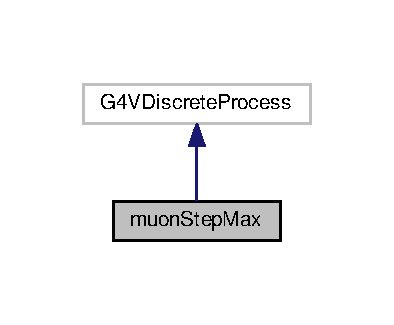
\includegraphics[width=189pt]{classmuonStepMax__inherit__graph}
\end{center}
\end{figure}


Collaboration diagram for muon\+Step\+Max\+:\nopagebreak
\begin{figure}[H]
\begin{center}
\leavevmode
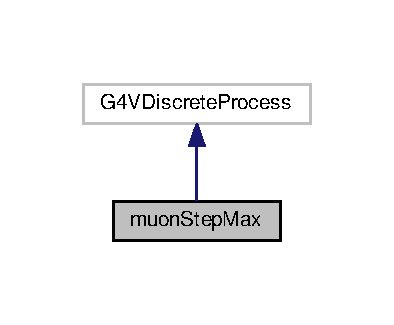
\includegraphics[width=189pt]{classmuonStepMax__coll__graph}
\end{center}
\end{figure}
\subsection*{Public Member Functions}
\begin{DoxyCompactItemize}
\item 
\mbox{\Hypertarget{classmuonStepMax_ae51ff3435957e85c269ef9d327b75482}\label{classmuonStepMax_ae51ff3435957e85c269ef9d327b75482}} 
{\bfseries muon\+Step\+Max} (const G4\+String \&process\+Name=\char`\"{}User\+Step\+Max\char`\"{})
\item 
\mbox{\Hypertarget{classmuonStepMax_a41ccffbc62f636553f3d9143e98b2079}\label{classmuonStepMax_a41ccffbc62f636553f3d9143e98b2079}} 
{\bfseries muon\+Step\+Max} (\hyperlink{classmuonStepMax}{muon\+Step\+Max} \&)
\item 
\mbox{\Hypertarget{classmuonStepMax_a4437a2282448452a419149cd8d8f7495}\label{classmuonStepMax_a4437a2282448452a419149cd8d8f7495}} 
virtual G4bool {\bfseries Is\+Applicable} (const G4\+Particle\+Definition \&)
\item 
\mbox{\Hypertarget{classmuonStepMax_a449cd30e5d5284d56a0dc10bf831e4db}\label{classmuonStepMax_a449cd30e5d5284d56a0dc10bf831e4db}} 
void {\bfseries Set\+Step\+Max} (G4double)
\item 
\mbox{\Hypertarget{classmuonStepMax_adf76383939936db76e310b661b4f332f}\label{classmuonStepMax_adf76383939936db76e310b661b4f332f}} 
G4double {\bfseries Get\+Step\+Max} ()
\item 
\mbox{\Hypertarget{classmuonStepMax_aea1aeac21f0095b44bedf878789b9d0d}\label{classmuonStepMax_aea1aeac21f0095b44bedf878789b9d0d}} 
virtual G4double {\bfseries Post\+Step\+Get\+Physical\+Interaction\+Length} (const G4\+Track \&track, G4double previous\+Step\+Size, G4\+Force\+Condition $\ast$condition)
\item 
\mbox{\Hypertarget{classmuonStepMax_af3da1fe21a53518e52fea709a52173fd}\label{classmuonStepMax_af3da1fe21a53518e52fea709a52173fd}} 
virtual G4\+V\+Particle\+Change $\ast$ {\bfseries Post\+Step\+Do\+It} (const G4\+Track \&, const G4\+Step \&)
\end{DoxyCompactItemize}
\subsection*{Protected Member Functions}
\begin{DoxyCompactItemize}
\item 
\mbox{\Hypertarget{classmuonStepMax_a792f2c77129ec1eeae9ac56902ec6e90}\label{classmuonStepMax_a792f2c77129ec1eeae9ac56902ec6e90}} 
G4double {\bfseries Get\+Mean\+Free\+Path} (const G4\+Track \&, G4double, G4\+Force\+Condition $\ast$)
\end{DoxyCompactItemize}


The documentation for this class was generated from the following files\+:\begin{DoxyCompactItemize}
\item 
include/muon\+Step\+Max.\+hh\item 
src/muon\+Step\+Max.\+cc\end{DoxyCompactItemize}

\hypertarget{classmuonSteppingAction}{}\section{muon\+Stepping\+Action类 参考}
\label{classmuonSteppingAction}\index{muon\+Stepping\+Action@{muon\+Stepping\+Action}}


stepping action 暂时没有做什么动作  




{\ttfamily \#include $<$muon\+Stepping\+Action.\+hh$>$}



类 muon\+Stepping\+Action 继承关系图\+:\nopagebreak
\begin{figure}[H]
\begin{center}
\leavevmode
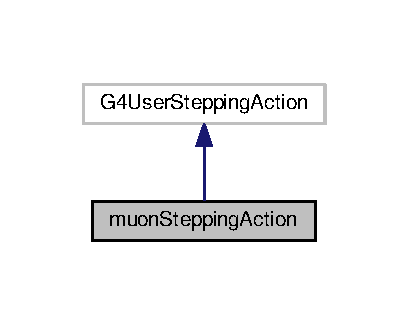
\includegraphics[width=196pt]{classmuonSteppingAction__inherit__graph}
\end{center}
\end{figure}


muon\+Stepping\+Action 的协作图\+:\nopagebreak
\begin{figure}[H]
\begin{center}
\leavevmode
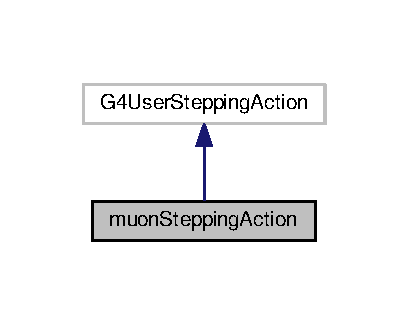
\includegraphics[width=313pt]{classmuonSteppingAction__coll__graph}
\end{center}
\end{figure}
\subsection*{Public 成员函数}
\begin{DoxyCompactItemize}
\item 
\hyperlink{classmuonSteppingAction_af61195514a24d468d05e62b421b360f1}{muon\+Stepping\+Action} (\hyperlink{classmuonEventAction}{muon\+Event\+Action} $\ast$event\+Action)
\item 
virtual \hyperlink{classmuonSteppingAction_a211068d7000014897633714af0f47b08}{$\sim$muon\+Stepping\+Action} ()
\item 
virtual void \hyperlink{classmuonSteppingAction_a8e1d7a65edc88bab12e7b0ff91ee7183}{User\+Stepping\+Action} (const G4\+Step $\ast$)
\end{DoxyCompactItemize}
\subsection*{Private 属性}
\begin{DoxyCompactItemize}
\item 
\hyperlink{classmuonEventAction}{muon\+Event\+Action} $\ast$ \hyperlink{classmuonSteppingAction_a79d6a211a68c4390cc75675876ad1a62}{f\+Event\+Action}
\end{DoxyCompactItemize}


\subsection{详细描述}
stepping action 暂时没有做什么动作 

在文件 muon\+Stepping\+Action.\+hh 第 18 行定义.



\subsection{构造及析构函数说明}
\mbox{\Hypertarget{classmuonSteppingAction_af61195514a24d468d05e62b421b360f1}\label{classmuonSteppingAction_af61195514a24d468d05e62b421b360f1}} 
\index{muon\+Stepping\+Action@{muon\+Stepping\+Action}!muon\+Stepping\+Action@{muon\+Stepping\+Action}}
\index{muon\+Stepping\+Action@{muon\+Stepping\+Action}!muon\+Stepping\+Action@{muon\+Stepping\+Action}}
\subsubsection{\texorpdfstring{muon\+Stepping\+Action()}{muonSteppingAction()}}
{\footnotesize\ttfamily muon\+Stepping\+Action\+::muon\+Stepping\+Action (\begin{DoxyParamCaption}\item[{\hyperlink{classmuonEventAction}{muon\+Event\+Action} $\ast$}]{event\+Action }\end{DoxyParamCaption})}



在文件 muon\+Stepping\+Action.\+cc 第 15 行定义.

\mbox{\Hypertarget{classmuonSteppingAction_a211068d7000014897633714af0f47b08}\label{classmuonSteppingAction_a211068d7000014897633714af0f47b08}} 
\index{muon\+Stepping\+Action@{muon\+Stepping\+Action}!````~muon\+Stepping\+Action@{$\sim$muon\+Stepping\+Action}}
\index{````~muon\+Stepping\+Action@{$\sim$muon\+Stepping\+Action}!muon\+Stepping\+Action@{muon\+Stepping\+Action}}
\subsubsection{\texorpdfstring{$\sim$muon\+Stepping\+Action()}{~muonSteppingAction()}}
{\footnotesize\ttfamily muon\+Stepping\+Action\+::$\sim$muon\+Stepping\+Action (\begin{DoxyParamCaption}{ }\end{DoxyParamCaption})\hspace{0.3cm}{\ttfamily [virtual]}}



在文件 muon\+Stepping\+Action.\+cc 第 19 行定义.



\subsection{成员函数说明}
\mbox{\Hypertarget{classmuonSteppingAction_a8e1d7a65edc88bab12e7b0ff91ee7183}\label{classmuonSteppingAction_a8e1d7a65edc88bab12e7b0ff91ee7183}} 
\index{muon\+Stepping\+Action@{muon\+Stepping\+Action}!User\+Stepping\+Action@{User\+Stepping\+Action}}
\index{User\+Stepping\+Action@{User\+Stepping\+Action}!muon\+Stepping\+Action@{muon\+Stepping\+Action}}
\subsubsection{\texorpdfstring{User\+Stepping\+Action()}{UserSteppingAction()}}
{\footnotesize\ttfamily void muon\+Stepping\+Action\+::\+User\+Stepping\+Action (\begin{DoxyParamCaption}\item[{const G4\+Step $\ast$}]{the\+Step }\end{DoxyParamCaption})\hspace{0.3cm}{\ttfamily [virtual]}}



在文件 muon\+Stepping\+Action.\+cc 第 27 行定义.



\subsection{类成员变量说明}
\mbox{\Hypertarget{classmuonSteppingAction_a79d6a211a68c4390cc75675876ad1a62}\label{classmuonSteppingAction_a79d6a211a68c4390cc75675876ad1a62}} 
\index{muon\+Stepping\+Action@{muon\+Stepping\+Action}!f\+Event\+Action@{f\+Event\+Action}}
\index{f\+Event\+Action@{f\+Event\+Action}!muon\+Stepping\+Action@{muon\+Stepping\+Action}}
\subsubsection{\texorpdfstring{f\+Event\+Action}{fEventAction}}
{\footnotesize\ttfamily \hyperlink{classmuonEventAction}{muon\+Event\+Action}$\ast$ muon\+Stepping\+Action\+::f\+Event\+Action\hspace{0.3cm}{\ttfamily [private]}}



在文件 muon\+Stepping\+Action.\+hh 第 28 行定义.



该类的文档由以下文件生成\+:\begin{DoxyCompactItemize}
\item 
include/\hyperlink{muonSteppingAction_8hh}{muon\+Stepping\+Action.\+hh}\item 
src/\hyperlink{muonSteppingAction_8cc}{muon\+Stepping\+Action.\+cc}\end{DoxyCompactItemize}

\hypertarget{classPMThit}{}\section{P\+M\+Thit类 参考}
\label{classPMThit}\index{P\+M\+Thit@{P\+M\+Thit}}


设置 pmt Hit 容器  




{\ttfamily \#include $<$P\+M\+Thit.\+hh$>$}



类 P\+M\+Thit 继承关系图\+:\nopagebreak
\begin{figure}[H]
\begin{center}
\leavevmode
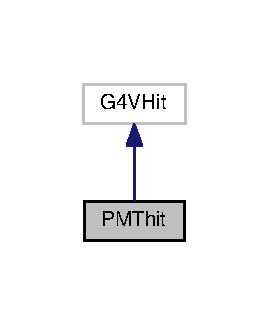
\includegraphics[width=129pt]{classPMThit__inherit__graph}
\end{center}
\end{figure}


P\+M\+Thit 的协作图\+:\nopagebreak
\begin{figure}[H]
\begin{center}
\leavevmode
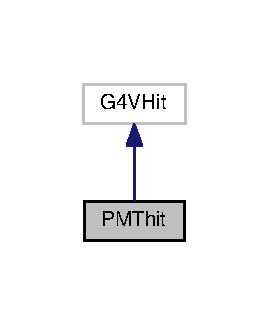
\includegraphics[width=129pt]{classPMThit__coll__graph}
\end{center}
\end{figure}
\subsection*{Public 成员函数}
\begin{DoxyCompactItemize}
\item 
void $\ast$ \hyperlink{classPMThit_a3a8f22237500cbebd0232e95c75d1983}{operator new} (size\+\_\+t)
\item 
void \hyperlink{classPMThit_a9f05cc06463bd5855188f47bcb8d36ee}{operator delete} (void $\ast$)
\item 
void \hyperlink{classPMThit_ae3dd4063284349849402f37858abbe64}{Set\+Delta\+Energy} (G4double deltaE)
\item 
void \hyperlink{classPMThit_a44d1262d477540bbc7084b49e9ac7a9f}{Set\+Time} (G4double time)
\item 
void \hyperlink{classPMThit_a87350831c86e7d49a9ee6a656246ec34}{Set\+Position} (G4\+Three\+Vector pos)
\item 
void \hyperlink{classPMThit_a4cd9d9b804e276177e9fd1d4200d2e70}{Set\+Name} (G4\+String name)
\item 
G4double \hyperlink{classPMThit_ac886469dc7bcc5e8f0d83de79fe636ee}{Get\+Delta\+Energy} () const
\item 
G4double \hyperlink{classPMThit_a0a9e1a55de9a3964babad3a5f81ad5bb}{Get\+Time} () const
\item 
G4\+Three\+Vector \hyperlink{classPMThit_ab731ac987db0650157d94673cd5a40be}{Get\+Position} () const
\item 
G4\+String \hyperlink{classPMThit_a497b90707c899f06ca4a1ecfdf537f64}{Get\+Name} () const
\end{DoxyCompactItemize}
\subsection*{Private 属性}
\begin{DoxyCompactItemize}
\item 
G4double \hyperlink{classPMThit_ab7d4a0178488f853b786a2acce0fccde}{f\+Delta\+Energy}
\item 
G4double \hyperlink{classPMThit_aeab761e89a1b0cb09f48a6009a2eed92}{f\+Time}
\item 
G4\+Three\+Vector \hyperlink{classPMThit_af2913329086e717fc91aa02748e1c646}{f\+Position}
\item 
G4\+String \hyperlink{classPMThit_a54a384bce361d05e46661879765acf6c}{fname}
\end{DoxyCompactItemize}


\subsection{详细描述}
设置 pmt Hit 容器 

Hit 容器保存能量,时间,位置,探测器名字 

在文件 P\+M\+Thit.\+hh 第 20 行定义.



\subsection{成员函数说明}
\mbox{\Hypertarget{classPMThit_ac886469dc7bcc5e8f0d83de79fe636ee}\label{classPMThit_ac886469dc7bcc5e8f0d83de79fe636ee}} 
\index{P\+M\+Thit@{P\+M\+Thit}!Get\+Delta\+Energy@{Get\+Delta\+Energy}}
\index{Get\+Delta\+Energy@{Get\+Delta\+Energy}!P\+M\+Thit@{P\+M\+Thit}}
\subsubsection{\texorpdfstring{Get\+Delta\+Energy()}{GetDeltaEnergy()}}
{\footnotesize\ttfamily G4double P\+M\+Thit\+::\+Get\+Delta\+Energy (\begin{DoxyParamCaption}{ }\end{DoxyParamCaption}) const\hspace{0.3cm}{\ttfamily [inline]}}



在文件 P\+M\+Thit.\+hh 第 32 行定义.

\mbox{\Hypertarget{classPMThit_a497b90707c899f06ca4a1ecfdf537f64}\label{classPMThit_a497b90707c899f06ca4a1ecfdf537f64}} 
\index{P\+M\+Thit@{P\+M\+Thit}!Get\+Name@{Get\+Name}}
\index{Get\+Name@{Get\+Name}!P\+M\+Thit@{P\+M\+Thit}}
\subsubsection{\texorpdfstring{Get\+Name()}{GetName()}}
{\footnotesize\ttfamily G4\+String P\+M\+Thit\+::\+Get\+Name (\begin{DoxyParamCaption}{ }\end{DoxyParamCaption}) const\hspace{0.3cm}{\ttfamily [inline]}}



在文件 P\+M\+Thit.\+hh 第 35 行定义.

\mbox{\Hypertarget{classPMThit_ab731ac987db0650157d94673cd5a40be}\label{classPMThit_ab731ac987db0650157d94673cd5a40be}} 
\index{P\+M\+Thit@{P\+M\+Thit}!Get\+Position@{Get\+Position}}
\index{Get\+Position@{Get\+Position}!P\+M\+Thit@{P\+M\+Thit}}
\subsubsection{\texorpdfstring{Get\+Position()}{GetPosition()}}
{\footnotesize\ttfamily G4\+Three\+Vector P\+M\+Thit\+::\+Get\+Position (\begin{DoxyParamCaption}{ }\end{DoxyParamCaption}) const\hspace{0.3cm}{\ttfamily [inline]}}



在文件 P\+M\+Thit.\+hh 第 34 行定义.

\mbox{\Hypertarget{classPMThit_a0a9e1a55de9a3964babad3a5f81ad5bb}\label{classPMThit_a0a9e1a55de9a3964babad3a5f81ad5bb}} 
\index{P\+M\+Thit@{P\+M\+Thit}!Get\+Time@{Get\+Time}}
\index{Get\+Time@{Get\+Time}!P\+M\+Thit@{P\+M\+Thit}}
\subsubsection{\texorpdfstring{Get\+Time()}{GetTime()}}
{\footnotesize\ttfamily G4double P\+M\+Thit\+::\+Get\+Time (\begin{DoxyParamCaption}{ }\end{DoxyParamCaption}) const\hspace{0.3cm}{\ttfamily [inline]}}



在文件 P\+M\+Thit.\+hh 第 33 行定义.

\mbox{\Hypertarget{classPMThit_a9f05cc06463bd5855188f47bcb8d36ee}\label{classPMThit_a9f05cc06463bd5855188f47bcb8d36ee}} 
\index{P\+M\+Thit@{P\+M\+Thit}!operator delete@{operator delete}}
\index{operator delete@{operator delete}!P\+M\+Thit@{P\+M\+Thit}}
\subsubsection{\texorpdfstring{operator delete()}{operator delete()}}
{\footnotesize\ttfamily void P\+M\+Thit\+::operator delete (\begin{DoxyParamCaption}\item[{void $\ast$}]{a\+Hit }\end{DoxyParamCaption})\hspace{0.3cm}{\ttfamily [inline]}}



在文件 P\+M\+Thit.\+hh 第 56 行定义.

\mbox{\Hypertarget{classPMThit_a3a8f22237500cbebd0232e95c75d1983}\label{classPMThit_a3a8f22237500cbebd0232e95c75d1983}} 
\index{P\+M\+Thit@{P\+M\+Thit}!operator new@{operator new}}
\index{operator new@{operator new}!P\+M\+Thit@{P\+M\+Thit}}
\subsubsection{\texorpdfstring{operator new()}{operator new()}}
{\footnotesize\ttfamily void $\ast$ P\+M\+Thit\+::operator new (\begin{DoxyParamCaption}\item[{size\+\_\+t}]{ }\end{DoxyParamCaption})\hspace{0.3cm}{\ttfamily [inline]}}



在文件 P\+M\+Thit.\+hh 第 47 行定义.

\mbox{\Hypertarget{classPMThit_ae3dd4063284349849402f37858abbe64}\label{classPMThit_ae3dd4063284349849402f37858abbe64}} 
\index{P\+M\+Thit@{P\+M\+Thit}!Set\+Delta\+Energy@{Set\+Delta\+Energy}}
\index{Set\+Delta\+Energy@{Set\+Delta\+Energy}!P\+M\+Thit@{P\+M\+Thit}}
\subsubsection{\texorpdfstring{Set\+Delta\+Energy()}{SetDeltaEnergy()}}
{\footnotesize\ttfamily void P\+M\+Thit\+::\+Set\+Delta\+Energy (\begin{DoxyParamCaption}\item[{G4double}]{deltaE }\end{DoxyParamCaption})\hspace{0.3cm}{\ttfamily [inline]}}



在文件 P\+M\+Thit.\+hh 第 27 行定义.

\mbox{\Hypertarget{classPMThit_a4cd9d9b804e276177e9fd1d4200d2e70}\label{classPMThit_a4cd9d9b804e276177e9fd1d4200d2e70}} 
\index{P\+M\+Thit@{P\+M\+Thit}!Set\+Name@{Set\+Name}}
\index{Set\+Name@{Set\+Name}!P\+M\+Thit@{P\+M\+Thit}}
\subsubsection{\texorpdfstring{Set\+Name()}{SetName()}}
{\footnotesize\ttfamily void P\+M\+Thit\+::\+Set\+Name (\begin{DoxyParamCaption}\item[{G4\+String}]{name }\end{DoxyParamCaption})\hspace{0.3cm}{\ttfamily [inline]}}



在文件 P\+M\+Thit.\+hh 第 30 行定义.

\mbox{\Hypertarget{classPMThit_a87350831c86e7d49a9ee6a656246ec34}\label{classPMThit_a87350831c86e7d49a9ee6a656246ec34}} 
\index{P\+M\+Thit@{P\+M\+Thit}!Set\+Position@{Set\+Position}}
\index{Set\+Position@{Set\+Position}!P\+M\+Thit@{P\+M\+Thit}}
\subsubsection{\texorpdfstring{Set\+Position()}{SetPosition()}}
{\footnotesize\ttfamily void P\+M\+Thit\+::\+Set\+Position (\begin{DoxyParamCaption}\item[{G4\+Three\+Vector}]{pos }\end{DoxyParamCaption})\hspace{0.3cm}{\ttfamily [inline]}}



在文件 P\+M\+Thit.\+hh 第 29 行定义.

\mbox{\Hypertarget{classPMThit_a44d1262d477540bbc7084b49e9ac7a9f}\label{classPMThit_a44d1262d477540bbc7084b49e9ac7a9f}} 
\index{P\+M\+Thit@{P\+M\+Thit}!Set\+Time@{Set\+Time}}
\index{Set\+Time@{Set\+Time}!P\+M\+Thit@{P\+M\+Thit}}
\subsubsection{\texorpdfstring{Set\+Time()}{SetTime()}}
{\footnotesize\ttfamily void P\+M\+Thit\+::\+Set\+Time (\begin{DoxyParamCaption}\item[{G4double}]{time }\end{DoxyParamCaption})\hspace{0.3cm}{\ttfamily [inline]}}



在文件 P\+M\+Thit.\+hh 第 28 行定义.



\subsection{类成员变量说明}
\mbox{\Hypertarget{classPMThit_ab7d4a0178488f853b786a2acce0fccde}\label{classPMThit_ab7d4a0178488f853b786a2acce0fccde}} 
\index{P\+M\+Thit@{P\+M\+Thit}!f\+Delta\+Energy@{f\+Delta\+Energy}}
\index{f\+Delta\+Energy@{f\+Delta\+Energy}!P\+M\+Thit@{P\+M\+Thit}}
\subsubsection{\texorpdfstring{f\+Delta\+Energy}{fDeltaEnergy}}
{\footnotesize\ttfamily G4double P\+M\+Thit\+::f\+Delta\+Energy\hspace{0.3cm}{\ttfamily [private]}}



在文件 P\+M\+Thit.\+hh 第 37 行定义.

\mbox{\Hypertarget{classPMThit_a54a384bce361d05e46661879765acf6c}\label{classPMThit_a54a384bce361d05e46661879765acf6c}} 
\index{P\+M\+Thit@{P\+M\+Thit}!fname@{fname}}
\index{fname@{fname}!P\+M\+Thit@{P\+M\+Thit}}
\subsubsection{\texorpdfstring{fname}{fname}}
{\footnotesize\ttfamily G4\+String P\+M\+Thit\+::fname\hspace{0.3cm}{\ttfamily [private]}}



在文件 P\+M\+Thit.\+hh 第 40 行定义.

\mbox{\Hypertarget{classPMThit_af2913329086e717fc91aa02748e1c646}\label{classPMThit_af2913329086e717fc91aa02748e1c646}} 
\index{P\+M\+Thit@{P\+M\+Thit}!f\+Position@{f\+Position}}
\index{f\+Position@{f\+Position}!P\+M\+Thit@{P\+M\+Thit}}
\subsubsection{\texorpdfstring{f\+Position}{fPosition}}
{\footnotesize\ttfamily G4\+Three\+Vector P\+M\+Thit\+::f\+Position\hspace{0.3cm}{\ttfamily [private]}}



在文件 P\+M\+Thit.\+hh 第 39 行定义.

\mbox{\Hypertarget{classPMThit_aeab761e89a1b0cb09f48a6009a2eed92}\label{classPMThit_aeab761e89a1b0cb09f48a6009a2eed92}} 
\index{P\+M\+Thit@{P\+M\+Thit}!f\+Time@{f\+Time}}
\index{f\+Time@{f\+Time}!P\+M\+Thit@{P\+M\+Thit}}
\subsubsection{\texorpdfstring{f\+Time}{fTime}}
{\footnotesize\ttfamily G4double P\+M\+Thit\+::f\+Time\hspace{0.3cm}{\ttfamily [private]}}



在文件 P\+M\+Thit.\+hh 第 38 行定义.



该类的文档由以下文件生成\+:\begin{DoxyCompactItemize}
\item 
include/\hyperlink{PMThit_8hh}{P\+M\+Thit.\+hh}\end{DoxyCompactItemize}

\hypertarget{classpmtSD}{}\section{pmt\+S\+D类 参考}
\label{classpmtSD}\index{pmt\+SD@{pmt\+SD}}


pmt的敏感探测器类  




{\ttfamily \#include $<$pmt\+S\+D.\+hh$>$}



类 pmt\+SD 继承关系图\+:\nopagebreak
\begin{figure}[H]
\begin{center}
\leavevmode
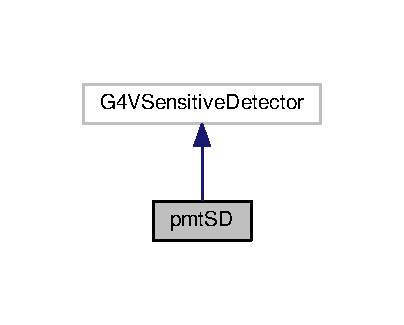
\includegraphics[width=194pt]{classpmtSD__inherit__graph}
\end{center}
\end{figure}


pmt\+SD 的协作图\+:\nopagebreak
\begin{figure}[H]
\begin{center}
\leavevmode
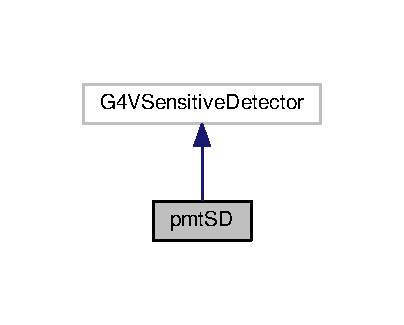
\includegraphics[width=194pt]{classpmtSD__coll__graph}
\end{center}
\end{figure}
\subsection*{Public 成员函数}
\begin{DoxyCompactItemize}
\item 
\hyperlink{classpmtSD_ae7746efb08ea75673a718fd342d243ea}{pmt\+SD} (G4\+String name)
\begin{DoxyCompactList}\small\item\em 设置敏感探测器保存哪些数据 \end{DoxyCompactList}\item 
void \hyperlink{classpmtSD_a5241646bdc0f46e27b011bf4fa35dc07}{Initialize} (G4\+H\+Cof\+This\+Event $\ast$) override
\end{DoxyCompactItemize}
\subsection*{Protected 成员函数}
\begin{DoxyCompactItemize}
\item 
G4bool \hyperlink{classpmtSD_a5d557bd42f85305418f6ddd7e4bcfe7a}{Process\+Hits} (G4\+Step $\ast$a\+Step, G4\+Touchable\+History $\ast$R\+Ohist) override
\end{DoxyCompactItemize}


\subsection{详细描述}
pmt的敏感探测器类 

在文件 pmt\+S\+D.\+hh 第 10 行定义.



\subsection{构造及析构函数说明}
\mbox{\Hypertarget{classpmtSD_ae7746efb08ea75673a718fd342d243ea}\label{classpmtSD_ae7746efb08ea75673a718fd342d243ea}} 
\index{pmt\+SD@{pmt\+SD}!pmt\+SD@{pmt\+SD}}
\index{pmt\+SD@{pmt\+SD}!pmt\+SD@{pmt\+SD}}
\subsubsection{\texorpdfstring{pmt\+S\+D()}{pmtSD()}}
{\footnotesize\ttfamily pmt\+S\+D\+::pmt\+SD (\begin{DoxyParamCaption}\item[{G4\+String}]{name }\end{DoxyParamCaption})}



设置敏感探测器保存哪些数据 

muon 击中 pmt ,保存时间,能量,位置和击中哪一个 pmt 信息 敏感探测器挂载在敏感探测器管理类格式为 name/pmt\+\_\+energy\+\_\+time 
\begin{DoxyParams}{参数}
{\em name} & pmt 的名字 \\
\hline
\end{DoxyParams}


在文件 pmt\+S\+D.\+cc 第 13 行定义.



\subsection{成员函数说明}
\mbox{\Hypertarget{classpmtSD_a5241646bdc0f46e27b011bf4fa35dc07}\label{classpmtSD_a5241646bdc0f46e27b011bf4fa35dc07}} 
\index{pmt\+SD@{pmt\+SD}!Initialize@{Initialize}}
\index{Initialize@{Initialize}!pmt\+SD@{pmt\+SD}}
\subsubsection{\texorpdfstring{Initialize()}{Initialize()}}
{\footnotesize\ttfamily void pmt\+S\+D\+::\+Initialize (\begin{DoxyParamCaption}\item[{G4\+H\+Cof\+This\+Event $\ast$}]{hcof }\end{DoxyParamCaption})\hspace{0.3cm}{\ttfamily [override]}}



在文件 pmt\+S\+D.\+cc 第 76 行定义.

\mbox{\Hypertarget{classpmtSD_a5d557bd42f85305418f6ddd7e4bcfe7a}\label{classpmtSD_a5d557bd42f85305418f6ddd7e4bcfe7a}} 
\index{pmt\+SD@{pmt\+SD}!Process\+Hits@{Process\+Hits}}
\index{Process\+Hits@{Process\+Hits}!pmt\+SD@{pmt\+SD}}
\subsubsection{\texorpdfstring{Process\+Hits()}{ProcessHits()}}
{\footnotesize\ttfamily G4bool pmt\+S\+D\+::\+Process\+Hits (\begin{DoxyParamCaption}\item[{G4\+Step $\ast$}]{a\+Step,  }\item[{G4\+Touchable\+History $\ast$}]{R\+Ohist }\end{DoxyParamCaption})\hspace{0.3cm}{\ttfamily [override]}, {\ttfamily [protected]}}



在文件 pmt\+S\+D.\+cc 第 21 行定义.



该类的文档由以下文件生成\+:\begin{DoxyCompactItemize}
\item 
include/\hyperlink{pmtSD_8hh}{pmt\+S\+D.\+hh}\item 
src/\hyperlink{pmtSD_8cc}{pmt\+S\+D.\+cc}\end{DoxyCompactItemize}

%--- End generated contents ---

% Index
\backmatter
\newpage
\phantomsection
\clearemptydoublepage
\addcontentsline{toc}{chapter}{Index}
\printindex

\end{document}
